
\chapter{Úvod}
\label{chap:introduction}

Při pořizování 3D obrazových dat se muže v datech objevit nechtěný šum, např.  ve zdravotnictví při pořizování výpočetní tomografie či magnetické resonance. Tento šum lze odstranit pomocí speciálních filtrů \dots komplexnějšími z těchto filtrů, bilaterálním filtrem a non-local means filtrem, se zabývá tato práce. 

Cílem této práce je seznámení se zmíněnými filtry a optimalizačními technikami při zpracovávaní obrazu (filtraci) a následně vybrané filtry efektivně implementovat pro filtraci 3D obrazových dat.

Tato práce je rozdělena do 6 kapitol, kde \ref{chap:introduction}. kapitolou je tento úvod. Ve \ref{chap:theory}. kapitole je rozepsán teoretický základ nutný k návrhu a implementaci filtrů, tj. popis 3D obrazových dat v sekci \ref{sec:theory:volumetric_data} a popis bilaterálního filtru a non-local means filtru v sekcích \ref{sec:design:bl} a~\ref{sec:design:nlm}. Ve~\ref{chap:design}. kapitole se nachází rozbor optimalizačních technik pro filtraci dat (sekce \ref{sec:design:optimalization}) a návrhy modelu bilaterálního filtru (sekce \ref{sec:design:bl}) a modelu non-local means filtru (sekce \ref{sec:design:nlm}) s~běžnými i vlastními optimalizacemi. 
Kapitola \ref{chap:implementation} se pak zabývá implementací těchto filtrů -- tj. vybranými technologiemi a strukturou řešení v sekci \ref{sec:impl:technology}, implementací 3D obrazových dat v~sekci~\ref{sec:impl:volumetric_data} a rozhraním filtrů v sekci \ref{sec:impl:filter}. Kapitola je pak zakončena implementačními informacemi a zajímavostmi v sekci \ref{sec:impl:bl} pro bilaterální filtr a \ref{sec:impl:nlm} pro non-local menas filter. V \ref{chap:results}. kapitole se nachází testování implementovaných filtrů v prostředí popsaném v sekci~\ref{sec:results:testing}, na datech popsaných v sekci \ref{sec:results:data} a porovnání výsledků proti referenčním filtrům definovaných v sekci~\ref{sec:results:ref_filters}. Testování bilaterálního filtru se nachází v  sekci \ref{sec:results:bl} a testování non-local means filtru je rozepsané v sekci \ref{sec:results:nlm}. Práce je zakončena závěrečnou \ref{chap:conclusion}. kapitolou, ve které je osobní zhodnocení výsledků a nastíněn další možný vývoj či rozšíření tohoto projektu.

\chapter{Nelineární filtry}
\label{chap:theory}
Cílem této kapitoly je seznámit čtenáře s teoretickým základem nutným k pochopení návrhu (viz kapitola~\ref{chap:design}) a implementace (viz kapitola \ref{chap:implementation}) nelineárních filtrů pro 3D obrazová data, a to bilaterálního filtru a non-local means filtru. Kapitola se nejdřív v sekci \ref{sec:theory:volumetric_data} zaměří na 3D 
obrazová data (formát, možné využití \dots), které budou vstupem bilaterálního filtru a non-local means filtru. Kapitola pak pokračuje rozborem bilaterálního filtru (sekce \ref{sec:theory:bl}) a non-local means filtru (sekce \ref{sec:theory:nlm}) -- principy, matematický popis, parametry a časová složitost.

\section{3D obrazová data}
\label{sec:theory:volumetric_data}
Volumetrická či 3D obrazová data jsou data, která drží informace o konkrétním modelu ve třech rozměrech, což přináší více dostupných informací a jejich lepší interpretaci. Využití volumetrických dat je velmi rozšířeno ve zdravotnictví -- magnetická resonance (MRI sken), výpočetní tomografire (CT sken) \dots a dalších odvětvích.

Volumetrická data se skládají z voxelů poskládaných do trojrozměrného pole, kde voxel obsahuje intenzitu daného bodu (případně RGB). Volumetrická data se obvykle pořizují po snímcích, které jsou následně rekonstruovány do 3D pole, přičemž může být rozdíl v reálných mezerách mezi snímky a mezi pixely ve snímcích, proto se k volumetrickým datům přikládá meta informace o skutečném rozložení voxelů (tzv. True Size či Spacing).

\subsection*{Formáty uložení volumetrických dat}
Volumetrická data mohou být uložena kompaktně jako jeden soubor, nebo rozdělena po snímcích:

\begin{itemize}
    \item RAW data je formát, který obsahuje pouze kompaktní volumetrická data bez jakýchkoliv metadat -- pro další práci je nezbytné  dodat další informace (rozměry dat, datový typ voxelů \dots).
    \item NRRD (Nearly Raw Raster Data) je robustní formát pro ukládání kompaktních volumetrických dat, obsahuje možnosti ukládání jako oddělená data a metadata, datový typ voxelů, komprese dat, způsob ukládání dat (endianess) \dots a podporu pro množství metadat (viz dokumentace\footnote{\url{http://teem.sourceforge.net/nrrd/format.html}}). Umožňuje reprezentaci RAW dat dopsáním NRRD hlavičky se správnými metadaty.
    \item DICOM (Digital Imaging and Communications in Medicine) je rozšířený standard pro komunikaci a správu lékařských dat, a tedy i volumetrických dat. Volumetrická data ukládá a spravuje po snímcích (viz dokumentace\footnote{\url{https://dicom.nema.org/medical/dicom/current/output/html/part01.html}}).
\end{itemize}

\begin{figure} [H]
    \centering
    \label{fig:vol:foot}
    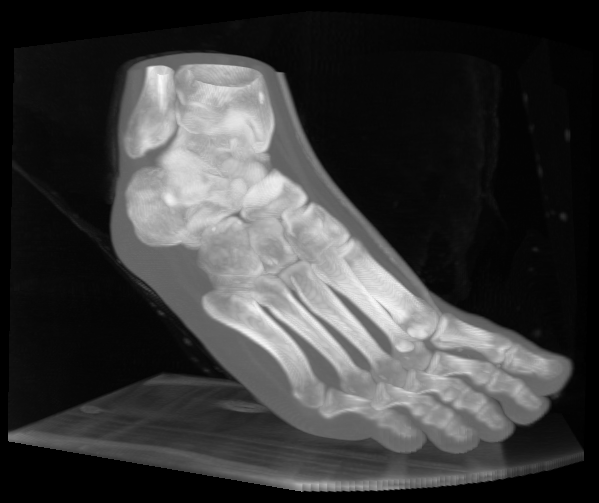
\includegraphics[width=0.60\textwidth]{figures/ct-foot.png}
    \caption{Ukázka volumetrických dat (výpočetní tomografie chodidla) vykreslených pomocí raycastingu.}
\end{figure}

\section{Bilaterální filtr}
\label{sec:theory:bl}
Durand a Dorsey \cite{bl2002:durand} popisují bilaterální filtr jako nelineární vyhlazovací filtr zachovávající hrany, jehož výstupem je vážený průměr vstupu. Váhy jednotlivých bodů závisí na dvou Gaussových funkcích. Vstupem první Gaussovy funkce je vzdálenost bodů (klasický Gaussův filtr), díky funkčním vlastnostem Gaussovy funkce se váhy nepočítají přes celý vstup, ale jen z blízkého okolí bodu. Vstupem druhé Gaussovy funkce je rozdíl intenzit bodů, což má za důsledek snížení vah bodů s velkým rozdílem intenzit, neboli vlastnost zachování hran (viz obrázek \ref{fig:bl:desc}).

\begin{figure} [H]
    \centering
    \label{fig:bl:desc}
    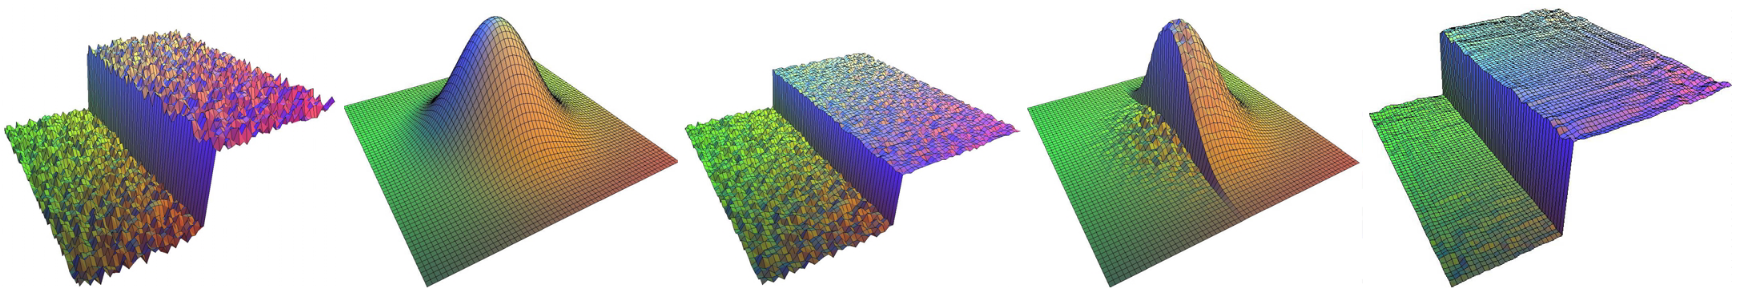
\includegraphics[width=1\textwidth]{figures/bf-dsc.png}
    \begin{tabularx}{1\textwidth}{
        >{\centering}X
        >{\centering}X
        >{\centering}X
        >{\centering}X
        >{\centering}X } 
        vstup & váhová funkce $G_{\sigma_s}$ & váhová funkce $G_{\sigma_r}$ & kombinace $G_{\sigma_s} \cdot G_{\sigma_r}$ & výstup
    \end{tabularx}
    \caption{Grafické znázornění průběhu bilaterálního filtrování, prostorové váhové funkce $G_{\sigma_s}$ a rozsahové váhové funkce $G_{\sigma_r}$ kolem centrálního bodu. Barvy jsou použity pouze pro demonstraci tvarů. \source{\cite{bl2002:durand}}}
\end{figure}

Bilaterální filtr je definován jako:
\begin{align}
    \label{eq:bf}
    I_{out}(x) &= \frac{1}{W_p}\displaystyle\sum_{x_i\in\Omega}I(x_i)G_{\sigma_r}(\|I(x_i)-I(x)\|)G_{\sigma_s}(\|x_i-x\|) \\
    W_p &= \displaystyle\sum_{x_i\in\Omega}G_{\sigma_r}(\|I(x_i)-I(x)\|)G_{\sigma_s}(\|x_i-x\|)
\end{align}

kde:
\begin{itemize}
    \item $I$ jsou vstupní data (obrazová data, volumetrická data)
    \item $I_{out}$ jsou výstupní (vyfiltrovaná) data
    \item $x$ jsou souřadnice právě filtrovaného bodu
    oblasti je $2r+1$
    \item $W_p$ je normalizační faktor
    \item $\Omega$ je množina bodů tvořící vyhledávací oblast (okno, krychle) se středem v bodě $x$, velikost oblasti závisí na parametru $r$, kde strana oblasti je $2r+1$
    \item $G_{\sigma_r}$ je rozsahová Gaussova funkce s parametrem $\sigma_r$ (tzv. range kernel)
    \item $\|I(x_i)-I(x)\|$ je absolutní hodnota rozdílu intenzit mezi právě filtrovaným bodem $x$ a bodem $x_i$, přes který je počítán vážený průměr
    \item $G_{\sigma_s}$ je prostorová Gaussova funkce s parametrem $\sigma_s$ (tzv. spatial/domain kernel)
    \item $\|x_i-x\|$ je  vzdálenost mezi právě filtrovaným bodem $x$ a bodem $x_i$, přes který je počítán vážený průměr
\end{itemize}

\subsection*{Parametry bilaterálního filtru}
Bilaterální filtr má 2 vstupní parametry -- $\sigma_r$ (tzv. range sigma) a $\sigma_s$ (tzv. spatial sigma), které jsou směrodatné odchylky Gaussových funkcí. Parametr $\sigma_r$ řídí rozsahovou Gaussovu funkci (závažnost rozdílu intenzit bodů) a parametr $\sigma_s$ řídí prostorovou Gaussovu funkci, tzn. řízení závažnosti vzdáleností bodů (viz obrázek \ref{fig:bf:grid}). Parametr $r$ (vstupní nebo vypočítaný z $\sigma_s$) udává velikost oblasti, přes kterou bilaterální filtr počítá vážený průměr. Jelikož velikost oblasti přímo ovlivňuje dobu filtrování, v praxi se proto parametr $r$ vybírá co nejmenší z rozmezí $(0;3\sigma_s\rangle$. Toto rozmezí je stanoveno pravidlem tří sigma \cite{wiki:3sigma}, které říká, že 99,73 \% nenulových hodnot normálního rozložení leží v rozmezí $\langle-3\sigma;3\sigma\rangle$, a tedy vážený průměr je počítaný přes 99,73 \% bodů s podstatně významnou vahou. Příliš malý parametr $r$ negativně ovlivňuje výsledek filtru.

\begin{figure} [H]
    \centering
    \label{fig:bf:grid}
    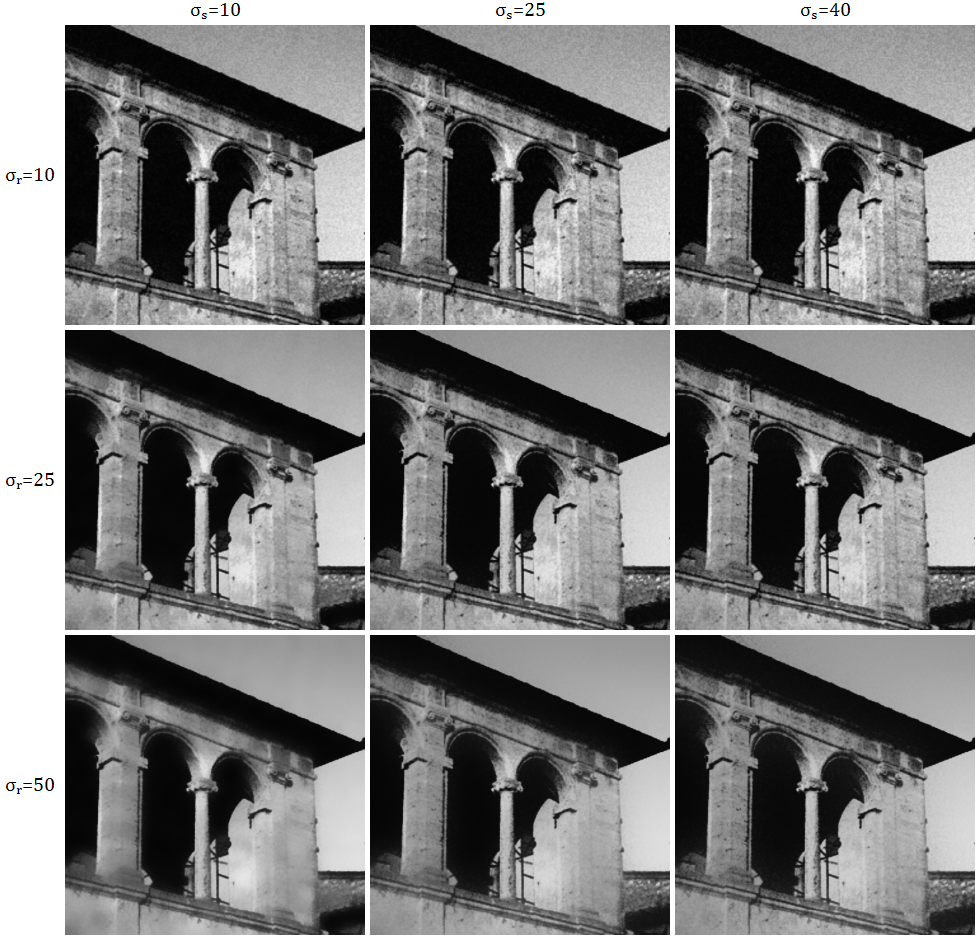
\includegraphics[width=1\textwidth]{figures/bf-grid.png}
    \caption{Vliv parametrů na výsledek bilaterálního filtrování.}
\end{figure}

\subsection*{Časová složitost}
\begin{tabularx}{1\textwidth}{ 
    >{\raggedright\arraybackslash}X 
    >{\raggedright\arraybackslash}X 
    >{\raggedright\arraybackslash}X }
    Vstupní data & Rozměry & Časová složitost \\
    \hline
    signál (1D) & $N$ & $\mathcal{O}(N \cdot (2r + 1))$ \\ 
    obrazová data (2D) & $W \times H$ & $\mathcal{O}(W \cdot H \cdot (2r + 1)^2)$ \\  
    volumetrická data (3D) & $W \times H \times D$ & $\mathcal{O}(W \cdot H \cdot D \cdot (2r + 1)^3)$
\end{tabularx}

\newpage

\section{Non-local means filtr}
\label{sec:theory:nlm}
Non-local means filtr prvně představil Buades \cite{nlm2005:buades} jako algoritmus, kde výstupní intenzita pixelu je počítána jako vážený průměr všech pixelů v obraze a nejen z blízkého okolí (odtud název non-local means). Váhy pixelů závisí na jejich podobnosti vůči vstupnímu pixelu, kde podobnost pixelů je souzena na základě okolí centrovaných kolem porovnávaného pixelu (viz obrázek \ref{fig:nlm:strategy}). Kvůli časové složitosti algoritmu jsou však podobné pixely vyhledávány jen v~předem definovaných vyhledávacích oblastech kolem filtrovaného pixelu.

\begin{figure} [H]
    \centering
    \label{fig:nlm:strategy}
    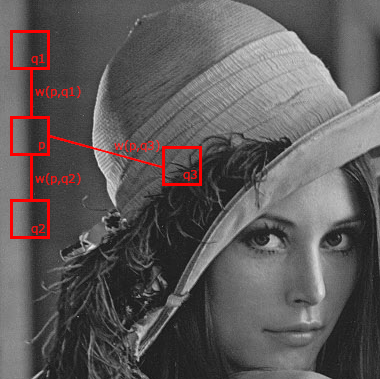
\includegraphics[width=0.6\textwidth]{figures/lena-nlm.png}
    \caption{Strategie non-local means filtru: podobné oblasti (kolem pixelů $q1$ a $q2$) vůči oblasti kolem vstupního pixelu $p$ vrátí vysoké váhy ($w(p,q1)$, $w(p,q2)$) a méně podobná oblast kolem pixelu $q3$ vrátí nižší váhu $w(p,q3)$. \source{\cite{nlm2005:buades}}}
\end{figure}

V původní verzi algoritmu \cite{nlm2005:buades} Buades počítal podobnosti okolí na základě vážené Euklidovské vzdálenosti intenzit jednotlivých pixeků v okolí, kde váhy odpovídají Gaussově funkci -- označuje se \texttt{NLM-Pa}, kde \texttt{a} připomíná využití vstupního parametru $a$ jako směrodatné odchylky Gaussovy funkce. Jacques Froment v \cite{nlm2014:froment} zmiňuje, že se v praxi gaussovská část často neimplementuje, jelikož přínos na výsledek filtrování, za cenu větší komplexnosti a dalšího parametru, je příliš malý. Filtr bez parametru $a$ se značí \texttt{NLM-P} a je definován jako: 
\begin{align}
    \label{eq:nlm}
    I_{out}(i) &= \frac{1}{Z(i)}\displaystyle\sum_{j\in\Omega}{I(j) \cdot w(i, j)} \\
    Z(i) &= \displaystyle\sum_{j\in\Omega}{w(i, j)} \\
    w(i, j) &= e^{-\frac{\|B(i) - B(j)\|_2^2}{h^2}}
\end{align}

kde:
\begin{itemize}
    \item $I$ jsou vstupní data (obrazová data, volumetrická data)
    \item $I_{out}$ jsou výstupní (vyfiltrovaná) data
    \item $i$ jsou souřadnice právě filtrovaného bodu
    \item $\Omega$ je vyhledávací oblast (okno, krychle) se středem v bodě $i$, tuto oblast filtr prohledává pro podobná okolí (patche), velikost vyhledávací oblasti je vstupním parametrem
    \item $Z(i)$ je normalizační faktor
    \item $w(i,j)$ je váhová funkce
    \item $B(p)$ je okolí kolem bodu $p$ (tzv. patch), jedná se o vektor intenzit bodů v okolí, velikost okolí je vstupním parametrem
    \item $\|B(i) - B(j)\|_2^2$ je  vzdálenost intenzit bodů v okolích $B(i)$ a $B(j)$
    \item $h$ je vstupní parametr řídící váhovou funkci
\end{itemize}

\subsection*{Parametry filtru non-local means}
Filtr \texttt{NLM-P} (běžná varianta klasického \texttt{NLM-Pa}) má 3 vstupní parametry, parametr $h$ řídící váhovou funkci, parametr $r$ nastavující velikost vyhledávacího okna, kde strana oblasti je $2r + 1$, a parametr $p$ řídící velikost patche, kde strana patche je $2p + 1$. Filtr \texttt{NLM-Pa} má další parametr $a$, který má pozitivně zlepšit vlastnosti filtru. 

\subsection*{Časová složitost}
Časová složitost klasického non-local means filtru je $\mathcal{O}(N \cdot (2r + 1)^d \cdot (2p + 1)^d)$, kde $N$ je velikost vstupních dat, $r$ je poloměr vyhledávací oblasti, $p$ je poloměr patche a $d$ je počet rozměrů vstupních dat (1D, 2D, 3D \dots). Složitost takového filtru je velká, proto byly navrženy přístupy pro zbavení závislosti časové složitosti na poloměru patche $p$, jedním z~přístupů, který je snadno rozšířitelný do 3D, je optimalizace pomocí integračního obrázku. Jacques Froment v \cite{nlm2014:froment} zmiňuje další 2 techniky -- využití FFT či sumy invariantních řádků (sum of invariant lines). 

\subsection*{Integrační obrázek}
\label{subsec:theory:nlm:integra_image}
Integrační obrázek je datová struktura a algoritmus pro rychlé a efektivní počítání ploch obdélníků v obrazových datech \cite{wiki:integral_image}. Pro rychlé spočítání je potřeba vstupní data nejdřív předpočítat do integračního obrázku, který má stejné rozměry jako vstupní data. Integrační obrázek pro 2D obrazová data je definovaný jako:

\begin{equation}
I(x, y) = \displaystyle\sum_{x'<x}{\displaystyle\sum_{y'<y}{i(x', y')}}
\end{equation}
kde $I(x, y)$ je hodnota integračního obrázku v bodě $[x, y]$ a $i(x', y')$ je intenzita obrazových dat v bodě $[x', y']$, konkrétní plochu $S$ ve 2D obrazových datech lze spočítat podle vzorce: 
\begin{equation}
    \label{eq:2dint:area}
    S = I(D) + I(A) - I(B) - I(C)
\end{equation}
kde obdélník plochy $S$ je dán počátečním bodem $[A_x + 1, A_y + 1]$ a koncovým bodem $[D_x, D_y]$ (viz obrázek \ref{fig:nlm:2d_integal_image}).

Z $N$ přístupů do paměti a $N - 1$ aritmetický operací (kde $N$ je počet bodů v obdélníku) je komplexnost získání obsahu $S$ snížena na 4 přístupy do paměti a 3 matematické operace, za cenu inicializace integračního obrázku a využité paměti.

\begin{figure} [H]
    \centering
    \label{fig:nlm:2d_integal_image}
    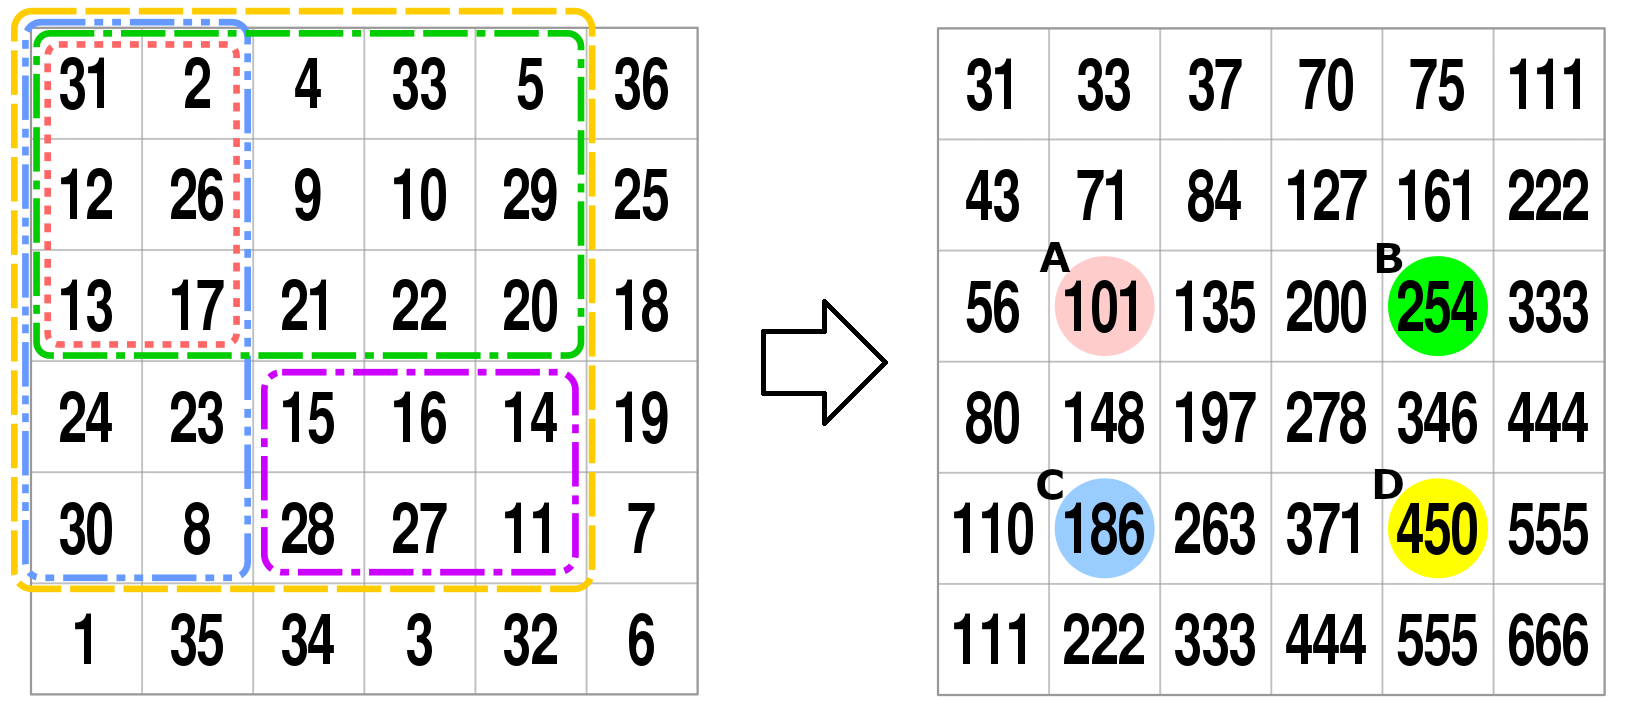
\includegraphics[width=0.85\textwidth]{figures/2d_integral_image.png}
    \caption{Ilustrace vztahu vstupních obrazových dat (vlevo) a integračního obrázku (vpravo). Barvy ve vstupních datech znázorňují plochy odpovídající hodnotám totožných barev v integračním obrázku, fialovou plochu lze spočítat vzorcem \ref{eq:2dint:area}. \source{\cite{wiki:integral_image}}}
\end{figure}

Integrační obrázek pro 2D obrazová data lze spočítat jedním průchodem vstupních dat dle vzorce:
\begin{equation}
    \label{eq:2dint:init}
    I(x, y) = I(x - 1, y) + I(x, y - 1) - I(x - 1, y - 1) + i(x, y)
\end{equation}
při průchodu daty směrem od počátečního bodu $[0,0]$ po koncový bod $[W, H]$, nejdřív je však nutné vypočítat hodnoty integračního obrázku podel os $x$ a $y$ dle vzorce:
$$I(p)=I(p-1)+i(p)$$
Při rozšíření integračního obrázku do 3D je kromě spočítáni os $x$, $y$, a $z$ nutné před konečným průchodem spočítat také roviny $xy$, $xz$ a $yz$, které se počítají obdobným způsobem jako 2D integrační obrázek (viz rovnice \ref{eq:2dint:init}). Konečný inicializační průchod 3D integračního obrázku je definován jako:
\begin{equation}
    I(x, y, z) = I(H) + I(C) - I(G) + I(B) - I(F) - I(A) + I(E) + i(x, y, z)
\end{equation}
kde $A$, $B$, $C$, $E$, $F$, $G$, $H$ jsou souřadnice reprezentující body v 3D prostoru (viz obrázek~\ref{fig:nlm:3d_integral_image}) a při inicializaci jsou definovány jako:
\begin{align*}
    A &= [x - 1, y - 1, z] \\
    B &= [x, y - 1, z] \\
    C &= [x - 1, y, z] \\
    D &= [x, y, z] \\
    E &= [x - 1, y - 1, z - 1] \\
    F &= [x, y - 1, z - 1] \\
    G &= [x - 1, y, z - 1] \\
    H &= [x, y, z - 1]    
\end{align*}
kde bod $D$ označuje právě počítanou hodnotu v 3D integračním obrázku.

\begin{figure} [H]
    \centering
    \label{fig:nlm:3d_integral_image}
    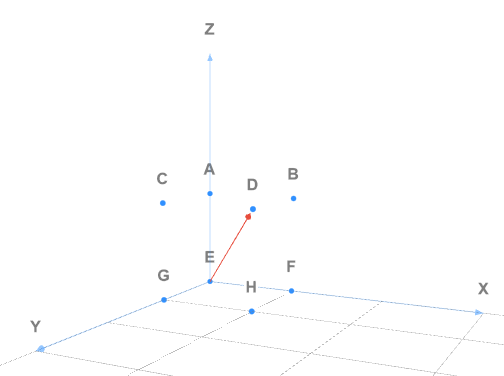
\includegraphics[width=0.9\textwidth]{figures/3d_integral_image.png}
    \caption{Ilustrace bodů při používání 3D integračního obrázku. Červený vektor zobrazuje směr vytváření integračního obrázku.}
\end{figure}

Objem $V$ konkrétní oblasti ve volumetrických datech lze spočítat dle vzorce:
\begin{equation}
    V = I(D) - I(H) + I(G) - I(C) + I(F) - I(E) + I(A) - I(B)
\end{equation}
kde oblast (kvádr) definující objem $V$ je daná počátečním bodem $[A_x + 1, A_y + 1, A_z + 1]$ a konečným bodem $[D_x, D_y, D_z]$, způsob uspořádání bodů $A-H$ v 3D prostoru je totožný způsobu v obrázku \ref{fig:nlm:3d_integral_image}.

Složitost získání objemu oblasti $V$ je tak snížena z $N$ přístupů do paměti a $N - 1$ aritmetických operací ($N$ je počet bodů v kvádru) na konstantních 8 přístupů do paměti a 7 matematický operací za cenu inicializace 3D integračního obrázku.

\chapter{Návrh řešení nelineárních filtrů pro 3D obrazová data}
\label{chap:design}
Tato kapitola se zabývá návrhem rychlých nelineárních filtrů (bilaterální filtr a non-local means filtr) pro 3D obrazová data. V kapitole jsou nejdříve rozebrány optimalizační techniky používané pro rychlé zpracování dat a filtraci (sekce \ref{sec:design:optimalization}). Dále je v kapitole, na základě teoretického základu z kapitoly \ref{chap:theory}, navržen model bilaterálního filtru (sekce \ref{sec:design:bl}) a model non-local means filtru s integračním obrázkem (sekce \ref{sec:design:nlm}), ve kterých jsou dříve zmíněné optimalizační techniky využity. 

\section{Optimalizační techniky}
\label{sec:design:optimalization}
Kromě zmenšení časové složitosti algoritmu lze rychlost filtrování optimalizovat technikami, které lépe využívají potenciálu počítače, na němž filtrování probíhá.

\subsection*{Paralelní zpracování}
Jednou z technik pro zrychlení zpracování je zpracovávat vstup paralelně na více jádrech procesoru, díky tomu je čas potřebný ke zpracování vstupu zkrácen počtem jader, v praxi je zrychlení o něco menší kvůli režii potřebné k přepínání kontextu mezi vlákny. U malých vstupních dat je možné, že režie vytváření vláken a přepínání kontextu předčí čas ušetřený paralelním zpracováním. Při zpracovávání na více vláknech je nezbytné vyhnout se co možná nejvíce konfliktům při přístupu k datům mezi vlákny, jelikož využití zámků vede k~častému přepínání kontextu, což může vést ke zpomalení zpracování vstupu.

Dalším přístupem pro paralelní zpracování dat je využití SIMD instrukcí (Single Instruction, Multiple Data), které využívají existence velkých datových SIMD registrů (128b, 256b) v moderních počítačích. Tyto registry umožňují přístup k několika číselným proměnným zároveň (tzv. vektory), a procesor tedy může provádět základní matematické operace (sčítání, násobení, dělení \dots) na vektorech, tzn. paralelně na číselných proměnných ve vektorech. 

\subsection*{Předpočítání parametrů a funkcí}
Filtraci popisují matematické rovnice, které v cyklu opakovaně počítají matematické výrazy, některé z parametrů těchto výrazů lze předpočítat jako koeficienty bez nutnosti je počítat při každé iteraci cyklu. Zvláště výhodné je předpočítat dělení koeficientem na násobení inverzním koeficientem (př. $f(x)=\frac{x}{\pi} \rightarrow f(x)=\frac{1}{\pi} \cdot x$), protože dělení je mnohem nákladnější operace než násobení. 

Pokud je znám možný rozsah vstupů funkce, je možné výsledky této funkce předpočítat do vyhledávací tabulky (tzv. looukup table), vstupy funkce se namísto výpočtu využijí pro indexaci ve vyhledávací tabulce. Pro přesné mapování vstupů na výstupy je potřeba, aby funkce měla celočíselné vstupy, pokud jsou vstupem desetinná čísla, nelze namapovat desetinný vstup na přesnou pozici a výsledek ve vyhledávací tabulce. Pro desetinné vstupy lze využít přibližné aproximující řešení funkce, tj. navzorkování funkce na $N$ vzorků, kde se desetinný vstup namapuje na nejbližší možný výstup ve vyhledávací tabulce (tzv. sampling). Počet vzorků ovlivňuje přenosnost aproximujícího řešení ke skutečnému. Předpočítání funkce je výhodné pokud se musí funkce často opakovat a pokud její provedení je dostatečně komplexní (mocnina, odmocnina, goniometrické funkce \dots).

\subsection*{Optimalizace kódu pro hardware}
Načítání dat z paměti je pomalé a každý přístup do paměti, který není uložený ve vyrovnávací paměti (cache), výrazně zpomaluje program. Proto je důležité zachovávat princip lokality dat a zpracovávat data přístupem, který tento princip dodržuje (tzv. cache-friendly). Běžným příkladem je zpracovávání vícerozměrného pole, kde prvky pole jsou fyzicky uloženy vedle sebe, ale logicky jsou poskládané do matice (ve 2D) \dots pro minimalizaci přístupů přímo do paměti (cache miss) je nutné správné pořadí vnořených cyklů přistupujících k prvkům ve vícerozměrném poli.

Dalším prvkem hardwaru, který může výrazně ovlivnit rychlost, je prediktor skoků (branch predictor). Prediktor skoků má za úkol dopředu předpovědět výsledek podmínky a díky tomu optimalizovat zpracovávání instrukcí, avšak pokud jsou vstupem podmínky špatně předpověditelná data (př. zašuměná obrazová data), předpověď skoku do špatné větve programu (branch misprediction) může stát hodně procesorového času, zvláště pokud je skok opakovaně špatně predikován ve vnořených smyčkách zpracovávajících $N$-rozměrná data (obrazová data, volumetrická data \dots). Omezení větvení programu může být obtížné, jednou z možností je nahrazení podmínky aritmetikou zajišťující stejný výsledek, která využívá způsobu ukládání čísel v paměti. Podmínky se objevují i ve vestavěných funkcích jako Min, Max, Abs \dots tohoto faktu lze využít u předpočítávání funkcí, kde může být výhodné předpočítat funkci i pro čísla mimo definovaný obor, tzn. předpočítání i pro záporné hodnoty symetrické funkce místo využití funkce absolutní hodnoty, předpočítání funkce za krajní hodnoty (padding) místo využití funkcí Min/Max \dots Příliš mnoho předpočítaných dat může negativně ovlivnit schopnost systému výhodně ukládat data do vyrovnávací paměti.

\newpage

\section{Rychlý bilaterální filtr a rozšíření do 3D}
\label{sec:design:bl}
Bilaterální filtr pro zápis do paměti využívá pouze lokální proměnné a příslušnou oblast výstupních dat, nedochází tedy ke konfliktu mezi vlákny a filtr je ideální pro paralelní zpracování. Pro filtrování barevných dat lze využít SIMD instrukce, které mohou zpracovat sdílenou část algoritmu pro RGB složky barev najednou a zmenšit tak faktor zpomalení filtru. 

Protože parametr $r$ ovlivňuje velikost průměrované oblasti, a tedy přímo ovlivňuje rychlost filtru, je výhodné zvolit co nejmenší hodnotu, která nemá negativní dopad na výsledek filtrování. Zvolením $r = 2,5\sigma_s$ lze dosáhnout slušného výsledku průměrovaného přes 98,7 \% nenulových hodnot \cite{wiki:integral_image} a výrazného zmenšení oblasti v porovnání s největším smysluplným parametrem $r = 3\sigma$ (viz obrázek \ref{fig:bf:3d_gauss}).

Váhy uvnitř cyklu jsou počítány pomocí dvou Gaussových funkcí -- prostorová $G_{\sigma_s}$ a rozsahová $G_{\sigma_r}$ (viz rovnice \ref{eq:bf}), Gaussovu funkci lze definovat jako $G_\sigma(x)=\exp(c \cdot x^2)$, kde $c=-\frac{0,5}{\sigma^2}$ je předpočítatelný koeficient. Předpočítání těchto funkcí je zásadní pro rychlé filtrování, neboť násobení spojené s matematickou funkcí $\exp$ je časové náročné na výpočet. 

\subsection*{Předpočítání rozsahové Gaussovy funkce}
Vstupem rozsahové funkce $G_{\sigma_r}$ je vzdálenost intenzit neboli absolutní hodnota rozdílu intenzit mezi vstupními body v datech. Pokud předpokládáme ukládání intenzity v obrazových datech na jednom bajtu (hodnoty 0-255), vstupem funkce pak může být vzdálenost v rozsahu 0-255, vyhledávací tabulka bude mít tedy 256 hodnot. Lze využít faktu, že absolutní hodnota dělá funkci symetrickou, a předpočítat i pro záporné vstupní hodnoty, vyhledávací tabulka pro rozsahovou Gaussovu funkci pak bude mít velikost 511 hodnot (255 záporných vstupů + 255 kladných vstupů + 1 vstup s nulovým rozdílem). Index do vyhledávací tabulky se pak spočítá jako $255 + I_1 - I_2$, kde $I_1$ a $I_2$ jsou intenzity porovnávaných bodů. Způsob předpočítání rozsahové Gaussovy funkce závisí na datovém typu reprezentující intenzitu, změna dimenze filtrujících dat tedy nijak nezmění tuto optimalizaci.

\subsection*{Předpočítání prostorové Gaussovy funkce}
Vstupem prostorové funkce $G_{\sigma_s}$ je  vzdálenost mezi body, protože výpočet vzdálenosti je časově náročný úkon (odmocnina, násobení) a výsledek je desetinné číslo, je výhodné Gaussovu funkci obalit novou funkcí $f$ a předpočítat ji. Pro 2D data je funkce $f$ definovaná jako:
\begin{align}
    \centering
    \label{eq:bl_space_lookup}
    f(x, y) &= G_{\sigma_s}(\sqrt{x^2 - y^2}) \\
    f(x, y) &= \exp(c \cdot (\sqrt{x^2 - y^2})^2) \\
    f(x, y) &= \exp(-\frac{0.5}{\sigma_s^2} \cdot (x^2 - y^2))
\end{align}
kde parametry $x = p_x - c_x$ a $y = p_y - c_y $ jsou posuny od centrálního pixelu $c$ k právě porovnávanému pixelu $p$. Obalení funkcí $f$ umožní předpočítat hodnoty pro celočíselná vstupní data ($x$ a $y$) v rozmezí $\langle-2,5\sigma_s;2,5\sigma_s\rangle$, vyhledávací tabulka bude tedy mít formát dvourozměrného pole, kde rozměry odpovídají rozměrům vyhledávací oblasti (viz obrázek~\ref{fig:bf:3d_gauss}). Pro 3D bilaterální filtr přibude souřadnice $z$ a vyhledávací tabulka bude mít formát 3D pole se stejným rozměry jako vyhledávací oblast (krychle kolem centrálního bodu $c$). Pro 3D bilaterální filtr může určení vzdálenosti být problém kvůli odlišným vzdálenostem mezi voxely způsobné druhem vytvoření volumetrických dat (viz volumetrická data \ref{sec:theory:volumetric_data}), běžným řešením je rozdílné vzdálenosti nezohledňovat. 

\begin{figure} [H]
    \centering
    \label{fig:bf:3d_gauss}
    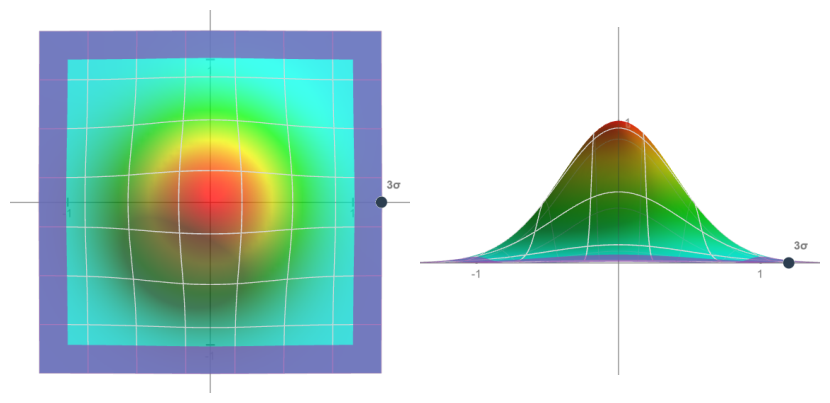
\includegraphics[width=1\textwidth]{figures/bf-3d-gauss-1.png}
    \caption{Ilustrace předpočítaných vah Gaussovy funkce pro 2D bilaterální filtr. Fialová oblast označuje ušetřenou oblast při použití parametru $r = 2,5\sigma_s$}
\end{figure}

\subsection*{Předpočítání vyhledávací oblasti}
\label{subsec:bf:precomupte_bias}
Z principu bilaterálního filtru, který předpokládá podobnost bodů na základě jejich vzdálenosti, se prostorová Gaussova funkce předpočítává jen do hranice $x^2+y^2=r^2$ a zbylé váhy ve vyhledávací tabulce zůstanou nulové, což zajistí, že váhy budou záviset pouze na vzdálenosti mezi porovnávanými body a ne na jejich pozici vůči sobě. Protože nulové body nemění nijak váhu, navrhuji je neprocházet vůbec a předpočítat vyhledávací oblast jako kruh (viz obrázek \ref{fig:bf:3d_gauss_bias}), to umožní snížit časovou složitost algoritmu z $\mathcal{O}(WH\cdot(2r+1)^2)$ na $\mathcal{O}(WH\cdot\frac{\pi}{4}(2r+1)^2)$, kde předpočítání vyhledávací oblasti znamená nastavení okrajů cyklu procházejícího vyhledávací oblast a předpočítání komplexních funkcí definující tyto okraje, tzn. $y \in \langle-r;r\rangle$ a $x \in \langle-\sqrt{r^2 - y^2};\sqrt{r^2 - y^2}\rangle$. Komplexní funkci definující okraje souřadnice $x$ lze předpočítat do 1D vyhledávací tabulky a zbavit se tak složitých operací násobení a odmocňování.

\begin{figure} [H]
    \centering
    \label{fig:bf:3d_gauss_bias}
    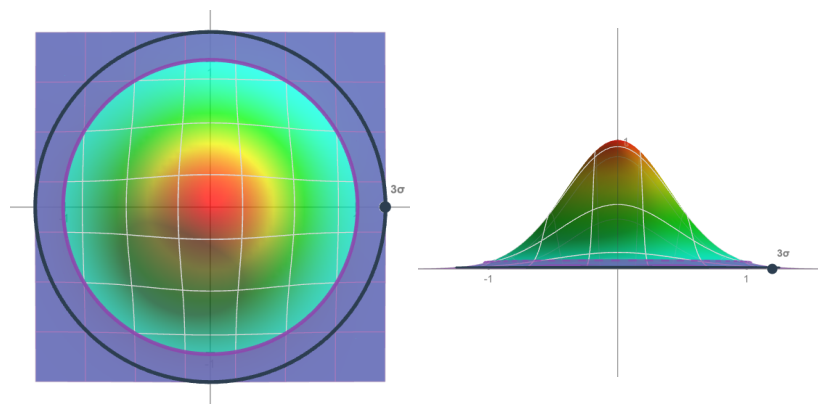
\includegraphics[width=1\textwidth]{figures/bf-3d-gauss-2.png}
    \caption{Ilustrace předpočítaných vah Gaussovy funkce pro 2D bilaterální filtr. Fialová oblast v rozmezí $x^2+y^2>=(2,5\sigma)^2$ označuje nízké váhy, které je možno vyřadit z váženého průměru bez vážného dopadu na výsledek filtrování, ale s výrazným dopadem na zrychlením algoritmu.}
\end{figure}

Při rozšíření filtru do 3D  (viz obrázek \ref{fig:bf:3d_bias}) se prostorová Gaussova funkce předpočítá pouze po hranici $x^2+y^2+z^2=r^2$, a okraje cyklu budou tedy definované jako:
\begin{align*}
    \centering
    x & \in \langle-r,r\rangle \\
    y & \in \langle-\sqrt{r^2-x^2};\sqrt{r^2-x^2}\rangle \\
    z & \in \langle-\sqrt{r^2-x^2-y^2};\sqrt{r^2-x^2-y^2}\rangle
\end{align*}

Komplexní funkci definující okraje souřadnice $y$ lze předpočítat do 1D vyhledávací tabulky obsahující posuny hranic počítaných ze souřadnice $x$. Komplexní funkce definující okraje souřadnice $z$ pak lze předpočítat do 2D vyhledávací tabulky obsahující posuny hranic počítaných ze souřadnic $x$ a $y$. Časová složitost je tedy snížena z $\mathcal{O}(WHD\cdot(2r+1)^3)$ na $\mathcal{O}(WHD\cdot\frac{\pi}{6}(2r+1)^3)$ a nejsou použity složité operace násobení, odmocnina \dots pro počítání okrajů vyhledávací oblasti.

\begin{figure} [H]
    \centering
    \label{fig:bf:3d_bias}
    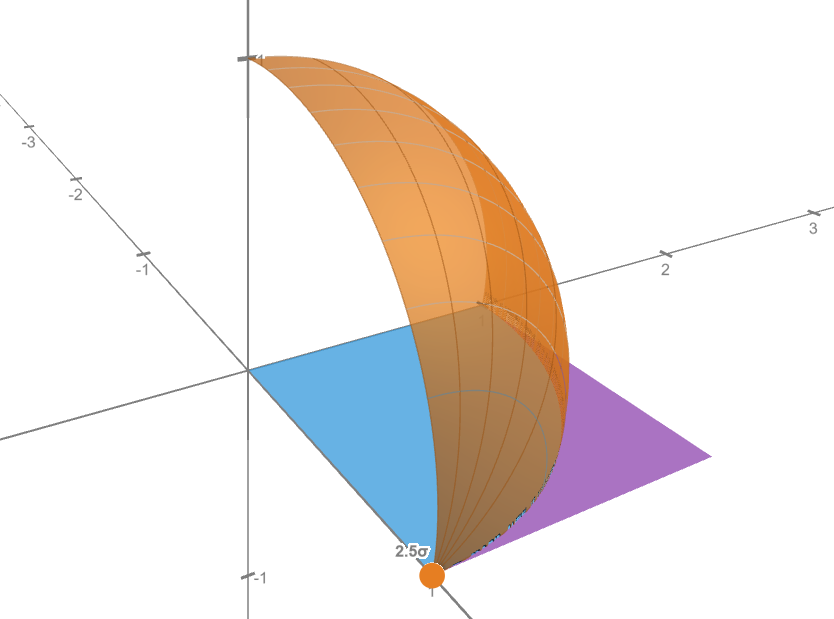
\includegraphics[width=0.6\textwidth]{figures/bf-3d-bias.png}
    \caption{Ilustrace hranice prohledávací oblasti $\Omega$ pro 3D bilaterální filtr. Modrá oblast označuje vysoké váhy Gaussovy funkce ve 2D (prohledávací oblast $\Omega$), fialová oblast označuje ušetřenou část Gaussovy funkce ve 2D s nízkými (nulovými) váhami. Oranžová oblast, definovaná jako $f(x,y)=\sqrt{r^2-x^2-y^2}$ a $r=2,5\sigma_s$, zobrazuje hranici mezi modrou a fialovou oblastí při rozšíření do 3D.}
\end{figure}

\subsection*{Překračování hranic obrazových dat}
Protože při počítání váženého průměru bodů na okraji obrazových dat dochází k překračování hranic (viz obrázek \ref{fig:bf:gauss_out_of_image_bounds}), je nutné vstupní data obalit vrstvou (tzv. padding), která většinou obsahuje barvu od nejbližšího okraje. Gaussova funkce může přesáhnout okraj až o $r$ bodů, takže data jsou vycpána $r$ body ve všech směrech (6 směrů ve 3D). 

\begin{figure} [H]
    \centering
    \label{fig:bf:gauss_out_of_image_bounds}
    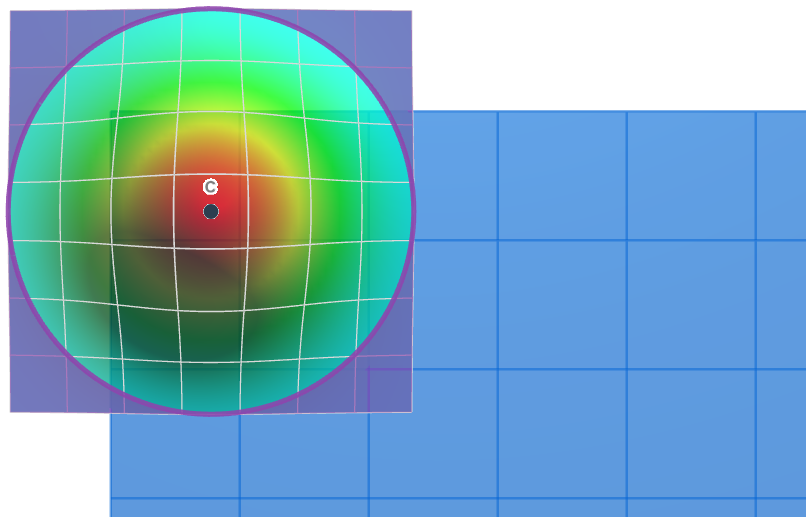
\includegraphics[width=0.80\textwidth]{figures/bf-gauss-out-of-bounds.png}
    \caption{Ilustrace prostorové Gaussovy funkce přesahující hranice 2D obrazových dat (modrá oblast) v okamžik filtrování pixelu v bodě $c$.}
\end{figure}

Alternativou je data neobalovat, ale využít funkce Min a Max pro převedení souřadnic mimo data na souřadnice nejbližšího okraje. Tyto dvě funkce lze spojit do jedné složené funkce definované jako:
\begin{equation*}
    f(x) =
        \begin{cases} 
            0 & x\leq 0 \\
            x & 0<x<N \\
            N-1 & N\leq x 
       \end{cases}
\end{equation*}
kde $x\in\langle-r;N+r\rangle$ jsou souřadnice v obrazových datech a $N$ je rozměr dat podél dané osy, díky tom, že je znám rozsah vstupních data, lze tuto funkci předpočítat do vyhledávací tabulky a zbavit se tak funkcí Min a Max, které mohou způsobit špatné predikce skoků (branch missprediction -- viz sekce \ref{sec:design:optimalization}). Předpočítat funkci $f(x)$ je nutné pro všechny souřadnice ($x$, $y$ a $z$ pro 3D), předpočítaná data budou mít formát 1D pole o velikosti $N + 2r$ (viz tabulka~\ref{tab:clamp_func}), kde $N$ odpovídá rozměru obrazových dat podél určité osy, pro transformaci vstupních souřadnic na indexy slouží vzorec: $index = x + r$. 

\begin{table} [H]
    \centering
    \label{tab:clamp_func}
    \begin{tabular}{|c|c|c|c|c|c|c|c|c|c|c|c|c|c|c|c|c|c|c|c|c|}
        \hline
        $x$ & \cellcolor{red!25}-4 & \cellcolor{red!25}-3 & \cellcolor{red!25}-2 & \cellcolor{red!25}-1 &
        0 & 1 & 2 & 3 & 4 & 5 & 6 & 7 & 8 & 9 & 10 &
        \cellcolor{red!25}11 & \cellcolor{red!25}12 & \cellcolor{red!25}13 & \cellcolor{red!25}14\\
        \hline
        index & 0 & 1 & 2 & 3 & 4 & 5 & 6 & 7 & 8 & 9 & 10 & 11 & 12 & 13 & 14 & 15 & 16 & 17 & 18\\
        \hline
        $f(x)$ & 0 & 0 & 0 & 0 & 0 & 1 & 2 & 3 & 4 & 5 & 6 & 7 & 8 & 9 & 10 & 10 & 10 & 10 & 10\\
        \hline
    \end{tabular}
    \caption{Tabulka předpočítané funkce složené z funkcí Min a Max, kde 1. řádek obsahuje vstupní souřadnice, 2. řádek obsahuje indexy, na které jsou vstupní souřadnice mapovány, a na 3. řádku jsou výstupní (předpočítané) souřadnice. Červené buňky znázorňují vstupní souřadnice mimo obrazová data.}
\end{table}

\subsection*{Paměťové nároky a časová složitost 3D bilaterálního filtru}
\begin{table} [H]
    \centering
    \begin{tabular}{|c|c|}
        \hline
        vstupní volumetrická data & $WHD \cdot S_{Byte}$ \\
        výstupní volumetrická data & $WHD \cdot S_{Byte}$ \\
        \hline
        předpočítaná rozsahová Gaussova funkce & $2 \cdot 255 + 1$ \\
        předpočitaná prostorová Gaussova funkce & $(2r + 1)^3 \cdot S_{Double}$ \\
        předpočítané okraje průměrované oblasti podél osy $y$ & $(2r + 1) \cdot S_{Double}$ \\
        předpočítané okraje průměrované oblasti podél osy $z$ & $(2r + 1)^2 \cdot S_{Double}$ \\
        předpočítané hranice volumetrických dat podél osy $x$ & $(W + 2r) \cdot S_{Double}$ \\
        předpočítané hranice volumetrických dat podél osy $y$ & $(H + 2r) \cdot S_{Double}$ \\
        předpočítané hranice volumetrických dat podél osy $z$ & $(D + 2r) \cdot S_{Double}$ \\
        \hline
    \end{tabular}
    \caption{Paměťové nároky (paměť alokovaná na haldě) navrženého 3D bilaterálního filtru. První část tabulky obsahuje nezbytná data pro filtraci, 2. část tabulky obsahuje předpočítaná data. Koeficient $S_{Byte}$ reprezentuje velikost 1 bajtu v paměti, $S_{Double}$ reprezentuje velikost desetinného čísla v paměti (double precision).}
\end{table}

Časová složitost navrženého filtru je $\mathcal{O}(WHD\cdot\frac{\pi}{6}(2r+1)^3)$ což je přibližně $2\times$ menší časová složitost ($\frac{\pi}{6}\approx0,52$) než původních $\mathcal{O}(WHD\cdot(2r+1)^3)$.

\newpage

\section{Rychlý non-local means filtr a rozšíření do 3D}
\label{sec:design:nlm}
Při zpracovávání non-local means filtrem, podobně jako u bilatelárního filtru, jsou paralelní zápisy do paměti nekonfliktní a lze tedy paralelně filtrovat bez použití zámků. Časová složitost klasického non-local means filtru závisí na velikosti patche a velikosti vyhledávací oblasti (viz non-local means filtr \ref{sec:theory:nlm}), závislosti na velikosti patche se dá zbavit použitím integračního obrázku. Pro rychlé filtrování je také nezbytné předpočítání váhové funkce, která se používá pro určování podobnosti patchů. 

\subsection*{Využití integračního obrázku}
Podobnost patche je počítaná na základě Euklidovské vzdálenosti, která je definovaná jako:
\begin{align}
    \label{eq:euclidien_distance}
    d(k,l)^2 &= (k[1] - l[1])^2 + (k[2] - l[2])^2 + \dots + (k[N] - l[N])^2 \\
    d(k,l)^2 &= \displaystyle\sum_{i=1}^N{(k[i] - l[i])^2}
\end{align}
kde $d(k,l)$ je  vzdálenost mezi vektory intenzit $k$ a $l$, $N$ je velikost vektoru (počet bodů v~patchi) -- $(2p + 1)^2$ ve 2D a $(2p + 1)^3$ ve 3D. Použitím integračního obrázku lze z algoritmu odstranit tyto sumy obdélníků/kvádů (viz integrační obrázek v sekci \ref{subsec:theory:nlm:integra_image}), tzn. odstranění závislosti na velikosti patche z časové složitosti filtru. Protože se ve vzorci~\ref{eq:euclidien_distance} kromě sčítání a odečítání také násobí, je využití integračního obrázku komplikované.

Jak zmiňuje Jacques Froment v \cite{nlm2014:froment}, je potřeba lehce upravit algoritmus filtru a předpočítat integrační obrázek pro každý možný vektor posunu ve vyhledávacím okně, kde místo intenzity budou integrační obrázky obsahovat součty rozdílů intenzit na druhou, tzn. že vzorec inicializace 2D integračního obrázku bude pozměněn na:
\begin{equation}
    I_{n}(x,y) = I_{n}(x-1,y)+I_{n}(x,y-1)-I_{n}(x-1,y-1)+(i(x,y)-i(x+t_x,y+t_y))^2
\end{equation}
kde $I_{n}$ je integrační obrázek, $n\in\langle0,N\rangle$ je index integračního obrázku a $N$ je počet integračních obrázků. $(t_x,t_y)$ je vektor posunu ve vyhledávací oblasti a $i(x,y)$ je intenzita obrazových dat v bodě $[x,y]$. Obdobně se změní inicializace 3D integračního obrázku. Protože uložení počtu integračních obrázků $N = (2r + 1)^3$ ve 3D je velice paměťově náročné, lze prohodit smyčky procházení vyhledávací oblasti a procházení konkrétních bodů v datech a spočítat tak integrační obrázek pro každý vektor posunu při filtrování. Je však nutné ukládat váhy a normalizační faktory do předem definovaného pole a na konec filtru přidat konečný průchod daty, který vážené průměry normalizuje a uloží do výstupních dat.

Při paralelním zpracování je nezbytné, aby každé vlákno mělo alokovaný vlastní prostor pro integrační obrázek z důvodu konfliktů při inicializaci, protože každé vlákno přistupuje jen do konkrétní oblasti integračního obrázku, lze inicializovat jenom tuto konkrétní oblast integračního obrázku a zmenšit tak časovou složitost inicializace. 

\subsection*{Překračování okrajů obrazových dat}
Při prohledávaní prostoru pro podobné patche a následném porovnávání patchů algoritmus non-local means filtru může překročit okraje až o vzdálenost $r + p$, kde $r$ je polovina strany vyhledávací oblasti a $p$ je polovina strany patche. Proto je nutné vycpat obrazová data tzv. padddingem, tzn. obalit data vrstvou, která bude obsahovat data nejbližšího okraje dat. Velikost vrstvy je stejná jako maximální přesah okraje ($k = r + p$, kde $k$ je velikost paddingu). Tyto paddingy se využijí i pro integrační obrázky a ostatní pole ukládající stav filtrování.

\subsection*{Vzorkování váhové funkce}
\label{subsec:nlm:sampling}
Non-local means filtr obsahuje poměrné komplexní váhovou funkci (viz rovnice \ref{eq:nlm}), kterou lze zjednodušit na $w(d^2) = \exp(-\frac{d^2}{h^2})$ kde $d^2 = \|B(i) - B(j)\|_2^2$. Za předpokladu, že intenzita voxelu je reprezentována bajtovým celým číslem, lze předpokládat rozsah vstupního parametru $d^2 \in \langle0;(2p + 1)^3 \cdot 255^2\rangle$, kde $(2p + 1)^3$ je objem patche a $255^2$ je maximální  vzdálenost mezi 2 intenzitami. I přes fakt, že vzdálenost je celým číslem, předpočítání všech vstupů váhové funkce by bylo paměťově náročné, proto navrhuji tuto funkci navzorkovat a počet vzorků přidat mezi vstupní parametry.

Váhová funkce bude předpočítaná do 1D vyhledávací tabulky o velikosti $N$, kde vstupní parametr $N \leq (2p + 1)^3 \cdot 255^2$ je počet vzorků. Vzorkování začíná na $0$ a krok vzorku je $\frac{(2p + 1)^3 \cdot 255^2}{N}$. Mapování vstupní vzdálenosti na index probíhá dle vzorce $d^2 \cdot \frac{N}{(2p + 1)^3 \cdot 255^2}$, kde $\frac{N}{(2p + 1)^3 \cdot 255^2}$ je předpočítatelný parametr.

\subsection*{Paměťové nároky a časová složitost 3D non-local means filtru}
\begin{table} [H]
    \centering
    \begin{tabular}{|c|c|}
        \hline
        vstupní volumetrická data & $(W + 2k)(H + 2k)(D + 2k) \cdot S_{Byte}$ \\
        výstupní volumetrická data & $(W + 2k)(H + 2k)(D + 2k)
        \cdot S_{Byte}$ \\
        \hline
        3D integrační obrázek & $T \cdot (W + 2k)(H + 2k)(D + 2k) \cdot S_{Long}$ \\
        vážené průměry bodů & $(W + 2k)(H + 2k)(D + 2k) \cdot S_{Double}$ \\
        normalizační faktory bodů & $(W + 2k)(H + 2k)(D + 2k) \cdot S_{Double}$ \\
        navzorkovaná váhová funkce & $N \cdot S_{Double}$ \\
        \hline
    \end{tabular}
    \caption{Paměťové nároky (paměť alokovaná na haldě) navrženého 3D nonlocal means filtru s integračním obrázkem. Parametr $k = r + p$ označuje padding kolem volumetrických dat, parmatetr $N$ je počet vzorků a $T$ je počet vláken použitých pro filtrování. Konstanta $S_{Byte}$ reprezentuje velikost 8b celého čísla v paměti, $S_{Double}$ reprezentuje velikost 64b desetinného čísla (double precision) a $S_{Long}$ reprezentuje velikost 64b celého čísla.}
\end{table}

Časová složitost navrženého 3D non-local means filtru s integračním obrázkem je zjednodušena z puvůdních $\mathcal{O}(N \cdot (2r + 1)^3 \cdot (2p + 1)^3)$ na $\mathcal{O}((2r + 1)^3\cdot((W+r)(H+r)(D+r) + WHD))$, kde $(W+r)(H+r)(D+r)$ představuje časovou složitost vytváření 3D integračního obrázku, časová složitost konečného průchodu daty je $\mathcal{O}(WHD)$.

\chapter{Implementace nelineárních filtrů pro 3D obrazová data}
\label{chap:implementation}
Tato kapitola se zaměřuje na implementaci nelineárních filtrů dle modelů navržených v \ref{chap:design}. kapitole. Nejprve je v sekci \ref{sec:impl:technology} vysvětlena struktura řešení a zvolené technologie, následně je v sekci \ref{sec:impl:volumetric_data} rozebrána implementace volumetrických dat. Kapitola pokračuje návrhem rozhraní filtrů pro paralelní zpracování (sekce \ref{sec:impl:filter}) a nakonec jsou představeny implementace 3D bilaterálního filtru (sekce \ref{sec:impl:bl}) a 3D non-local means filtru (sekce \ref{sec:impl:nlm}).

\section{Vybrané technologie a struktura řešení}
\label{sec:impl:technology}
Pro programování jsem zvolil jazyk C\# a platformu .NET (dotnet). Dotnet poskytuje multiplatformní řešení pro knihovny, konzolové aplikace \dots Pro dotnet lze vyvinout i poměrně rychlé apliakce (viz dále) a jazyk C\# má kvalitní dokementaci a poměrné velký ekosystém vývojářů volně poskytujících open source knihovny (tzv. NuGet balíčky). Pro vývoj také lze využít Visual Studio, které obsahuje profiler výhodný k analýze výkonnosti aplikace a využití prostředků počítače. 

Řešení bylo vyvinuto pod .NET SDK 6.0 (Software development kit) a pro spuštění je vyžadován .NET runtime (min. 6.0). Kromě grafické demo aplikace (GUI -- Graphical user interface) jsou všechny moduly multiplatformní včetně konzolové demo aplikace (CLI -- Command-line interface). Při vývoji jsem využíval verzovacího systému Git -- veškeré zdrojové kódy včetně demo aplikací (GUI a CLI) a testovacího skriptu jsou dostupné online na mém osobním GitHubu\footnote{\url{https://github.com/skrasekmichael/NonlinearFilters}}.

\subsection*{Výkonné aplikace v .NET}
Dotnet aplikace jsou optimalizovány ve dvou krocích:
\begin{enumerate}
    \item při překladu zdrojového kódu do IL (Intermediate Language), který je nezávislý na platformě
    \item při překladu IL na platformou specifikovanou sadu instrukcí tzv. JIT (Just-in-Time) kompilátorem
\end{enumerate}
přičemž markantnější optimalizace provádí JIT.

Dotnet aplikace běží s GC (Garbage collector), který usnadňuje práci s pamětí a zajišťuje odstranění úniků paměti (memory leak), ale má negativní dopad na výkonnost aplikace. Díky GC je C\# bezpečný pro práci s pamětí a nabízí rozhraní \texttt{Span<T>} a \texttt{Memory<T>} pro efektivní a bezpečný přístup do paměti. C\# také nabízí možnost použití klíčového slova \texttt{unsafe} pro definování unsafe contextu ve kterém lze přistupovat do paměti \uv{nebezpečně} pomocí odkazů (pointerů) a využívat pointerovou aritmetiku. Využitím pointerové aritmetiky lze také dosáhnout odstraní kontroly indexu pole (tzv. array bounds check) -- i když JIT často dokáže odhadnout, kdy je nutné kontrolu indexu provádět, její odstranění může markantně zvýšit výkonnost. 

Preferovaným způsobem paralelizmu v dotnetu je využití TBL (Task Parallel Library), jejíž koncept je založen na úlohách (tasks) a využívá rozhraní \texttt{Task}. Dokumentace \cite{dotnet_doc:tbl} uvádí, že výhodou použití úloh je efektivnější a škálovatelnější využití systémových prostředků. I~když dotnet nabízí přístup ke klasickému rozhraní vlákna (\texttt{Thread}), využitím vyšší abstrakce úloh přináší větší kontrolou nad asynchronním programováním a bohatší API (Application programming interface) pro paralelní programování. 

Dotnet umožňuje paralení zpracování celých registrů pomocí datových typů zrychlených SIMD instrukcemi, tyto typy lze nalézt pod jemným prostorem \texttt{System.Numerics}, kde se nachází datové type pro vektory, matice, roviny \dots

\subsection*{Struktura repositáře}
\begin{itemize}
    \item README.md -- soubor se základními informacemi o projektu a výsledky měření filtrů v porovnání s referenčními filtry. 
    \item Sources -- veškeré zdrojové kódy rozděleny do modulů (v dotnetu tzv. projekty).
    \begin{itemize}
        \item NonlinearFilters -- knihovna s implementacemi 2D a 3D filtrů (bilaterální filtr a non-local means filtr) s možností paralelního zpracování.
        \item NonlinearFilters.Volume -- modul s rozhraním volumetrických dat a logikou pro načítání a ukládání dat v různých formátech.
        \item NonlinearFilters.APP -- projekt demonstrující využití knihovny s filtry v moderní grafické aplikaci (WPF framework).
        \item NonlinearFilters.APP.VolumeRender -- modul pro jednoduchý 3D rendering\footnote{raycasting impl. dle \url{https://www.willusher.io/webgl/2019/01/13/volume-rendering-with-webgl}} volumetrických dat pomocí NuGet balíčku OpenTK\footnote{OpenGL rozhraní pro C\#}.
        \item NonlinearFilters.CLI -- projekt demonstrující využití knihovny s filtry v konzolové aplikaci s CLI pro spouštění filtrů.
    \end{itemize}
    \item Data -- obsahuje příklady zašuměných vstupních 2D obrazových a volumetrických dat.
    \item Images -- složka s výstupními obrázky generovanými testovacím souborem, které jsou využity v README souboru.
    \item Python -- python skripty umožňující spouštění referenčních filtrů.
    \item test.ps1 -- testovací PowerShell skript, který testuje filtry pomocí CLI aplikace a porovnává výsledky a dobu zpracování s referenčními filtry. 
    \item ostatní soubory a složky -- Makefile, .gitignore \dots
\end{itemize}

\section{Implementace volumetrických dat}
\label{sec:impl:volumetric_data}
Volumetrická data jsou reprezentovaná třídou \texttt{VolumetricData} implementující parametry dat (rozměry, skutečná velikost \dots viz sekce \ref{sec:theory:volumetric_data}) a trojrozměrné pole voxelů. Předpokládaným vstupem filtrů jsou šedotónová volumterická data s intenzitou voxelu reprezentovanou na 8 bitech, tzn. pole voxelů je datového typu \texttt{byte[]} a index voxelu na pozici $[x, y, z]$ je vypočítán jako:
\begin{equation}
    \label{eq:3dindex}
    index = x \cdot H \cdot D + y \cdot D + z
\end{equation}
kde $H$ je výška dat a $D$ je hloubka dat. Vzorec \ref{eq:3dindex} (a filtry pracující s volumetrickými daty) předpokládá data uložená v paměti v pořadí $x$, $y$, $z$, kdy souřadnice $z$ se mění nejrychleji a $x$ nejpomaleji. Pokud jsou data serializovaná v pořadí $z$, $y$, $x$, je potřeba při čtení/zápisu dat u~parametru velikosti (případně u dalších parametrů) prohodit rozměr hloubky s šířkou, o to se stará třída obsluhující soubory, kde každý formát volumetrických dat (NRRD \dots) má dedikovanou třídu dědící z abstraktní třídy \texttt{BaseFileHandler}. Kromě prohození pořadí serializace můžou \uv{FileHandlery} formátů při čtení/zápisu data překonvertovat (př. z floatů na bajty), data komprimovat (gzip \dots) a obsloužit další parametry formátů volumetrických dat (skutečná velikost).
I když filtry nevyužívají parametru skutečné velikosti volumetrických dat, může tento parametr být využit při interpretaci (rendering \dots).

\section{Implementace rozhraní filtru}
\label{sec:impl:filter}
Filtr má 3 výpočetně náročné části:
\begin{itemize}
    \item Inicializace filtru -- předpočítá a inicializuje parametry nezávislé na parametrech filtrování, ale závislé na vstupní datech.
    \item Předpočítání parametrů -- předpočítá parametry nezávislé na vstupních datech, ale závislé na parametrech filtrování.
    \item Filtrování -- paralelně vyfiltruje vstupní data.
\end{itemize}
Všechny filtry dědí z generické abstraktní třídy \texttt{BaseFilter<T>}, která rozhraní těchto částí definuje, generický parametr \texttt{T} je datový typ parametrů filtru. Rozhraní 2D a 3D filtrů se mírně liší kvůli vstupním datům, 2D filtry dědí z \texttt{BaseFilter2<T>} a pracují s 2D obrazovými daty pomocí multiplatformního API poskytnuté NuGet balíčkem \texttt{ImageSharp}. 3D filtry dědí z \texttt{BaseFilter3<T>} a pracují s volumetrickými daty definovanými v sekci \ref{sec:impl:volumetric_data}. 

\subsection*{Kroky filtrování}
\begin{enumerate}
    \item Inicializuje se filtr, pokud dosud nebyl inicializován.
    \item Obalí se vstupní data paddingem a vytvoří se nová výstupní data s paddingem.
    \item Předpočítají se parametry, pokud dosud nebyly předpočítány nebo pokud se vstupní parametry filtru změnily.
    \item Rozdělí se vstupní data na sektory pro paralelní zpracování.
    \item Vytvoří a spustí se úlohy pro paralelní filtraci, každé úloze se přidělí sektor v datech pro filtrování. Úlohy jsou vytvořeny s možností \texttt{TaskCreationOptions.LongRunning}, která umožní lepší plánovaní vlákna.
    \item Po dokončení všech úloh se následně odstraní padding z vyfiltrovaných dat.
\end{enumerate}

\subsection*{Rozdělení dat}
Při paralelním filtrování je potřeba výstupní data rozdělit na neprotínající se sektory, aby při zápisu dat nedocházelo ke konfliktu. Kvůli zachování principu lokality (viz sekce \ref{sec:design:optimalization}) je výhodné data dělit podél nejpomaleji měnící se souřadnice -- podél osy $y$ pro 2D obrazová data a podél osy $x$ pro volumetrická data. Protože rozměr dat nelze vždycky celočíselně rozdělit, poslední sektor může být větší než ostatní sektory (viz obrázek \ref{fig:impl:split})

\begin{figure} [H]
    \centering
    \label{fig:impl:split}
    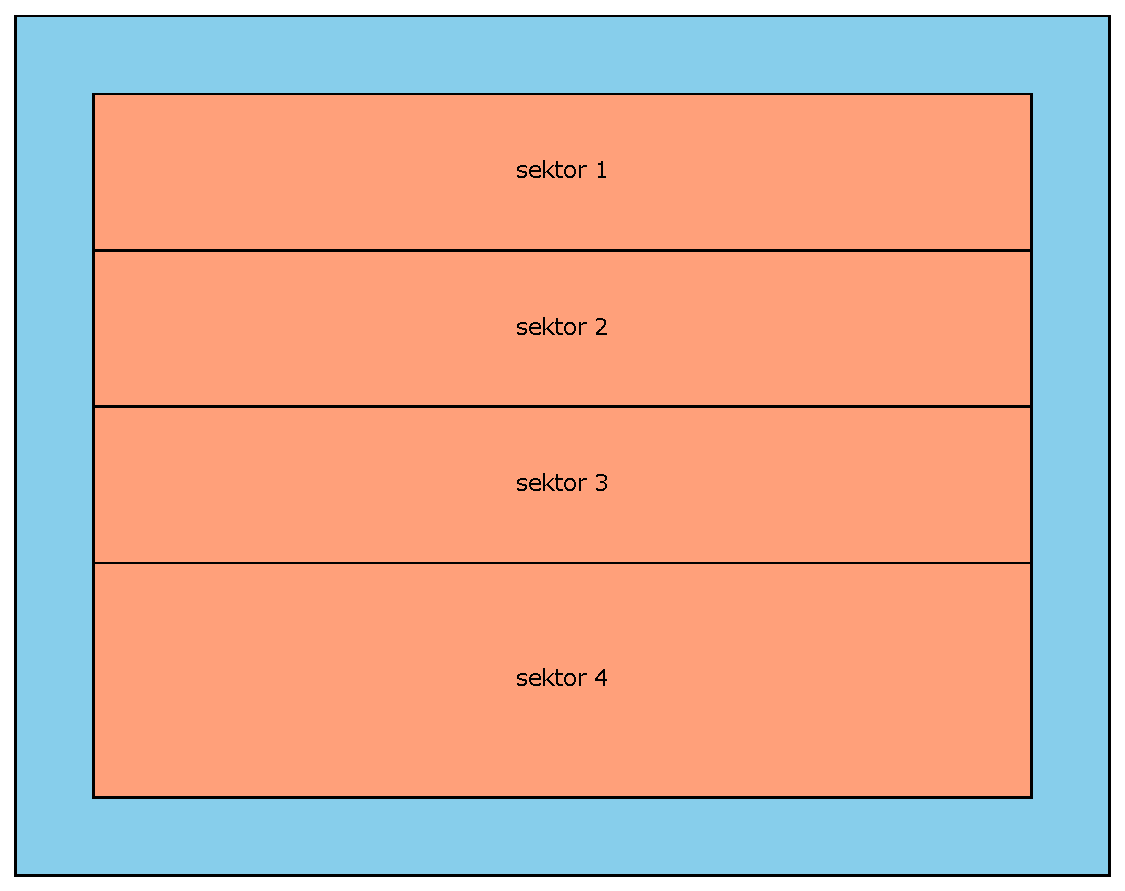
\includegraphics[width=0.80\textwidth]{figures/split.pdf}
    \caption{Ilustrace rozdělení 2D obrazových dat na sektory pro paralelní zpracování na 4 vláknech. Modrá barva označuje padding dat, který není potřeba filtrovat, červená barva označuje data rozdělená na sektory, kde každý sektor je přidělen úloze (vláknu).}
\end{figure}

\subsection*{Asynchronní filtr}
Při filtrování v okenních aplikacích se předpokládá nezamrznutí okna, tzn. použití asynchronního filtru, a zobrazení pokroku filtrování a případnou možnost zrušit filtrování (viz obrázek \ref{fig:impl:demo_cancel}).
Kvůli vyhnutí konfliktům si každé vlákno ukládá svůj postup (počet již vyfiltrovaných bodů) do pole na pozici odpovídající indexu sektoru/vlákna, filtr poté občas vyvolá událost \texttt{OnProgressChanged} s parametrem udávajícím procento vyfiltrovaných dat. Protože malá nepřesnost v postupu je bezvýznamná, lze celkový postup vypočítat bez použití zámků jako:
\begin{equation*}
    progress = \frac{1}{N} \cdot \displaystyle\sum_{i=0}^T{P[i]}
\end{equation*}
kde $N$ je počet bodů v obraze ($WH$ pro 2D, $WHD$ pro 3D), $T$ je počet vláken, na kterých je filtr spuštěn a $P$ je pole pro ukládání postupu jednotlivých vláken. 

Aby šlo filtrování kdykoli zrušit, musí každý filtr při filtraci kontrolovat stav vnitřní proměnné \texttt{IsCanceled}, která udává, zda bylo filtrování zrušeno. Filtr poté ukončí činnost filtrování a provede konečné kroky pro udržení konzistence dat.

\begin{figure} [H]
    \centering
    \label{fig:impl:demo_cancel}
    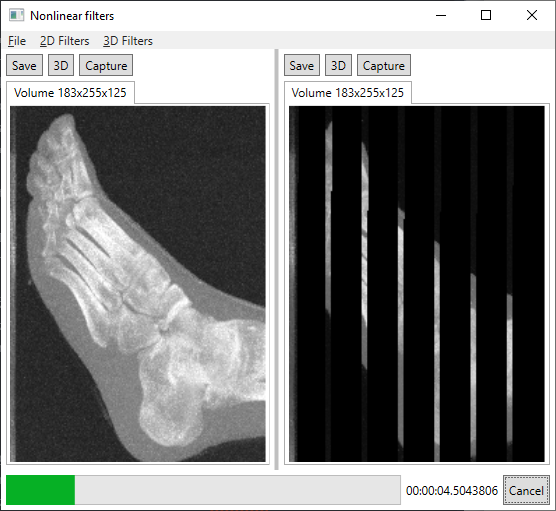
\includegraphics[width=1\textwidth]{figures/demo_cancel.png}
    \caption{Ukázka z demonstrační aplikace zobrazující funkci zrušení filtrace a zobrazení postupu filtrace. Obrázek vlevo jsou vstupní zašuměná volumetrická data. Obrázek vpravo ukazuje výsledek filtrace (bilaterální filtr) zrušené po 4,5 vteřinách, z obrázku je patrné paralelní zpracování -- 7 již vyfiltrovaných oblastí. Pod obrázky je \texttt{ProgressBar} zobrazující postup filtrování.}
\end{figure}

\pagebreak

\section{Implementace 3D bilaterálního filtru}
\label{sec:impl:bl}
Vstupními parametry filtrace modelem 3D bilaterálního filtru (viz sekce \ref{sec:design:bl}) jsou $\sigma_r$, $\sigma_s$ řídící váhové funkce a parametr $r$, který udává poloměr koule reprezentující relevantní váhy prostorové Gaussovy funkce (viz obrázek \ref{fig:bf:3d_gauss}). Pokud parametr $r$ není zadán, je parametr spočítán jako $r=2,5\sigma_s$. Navržený model 3D bilaterálního filtru nepoužívá padding dat, ale předpočítává hranice dat, tyto hranice lze jednoduše spočítat při inicializaci filtru:
\begin{verbatim}
border = new int[r + size + r];
for (int i = r; i < border.Length; i++) {
    border[i] = min(i - r, size - 1);
}
\end{verbatim} 
kde \texttt{border} je vyhledávací tabulka hraniční funkce, \texttt{r} je vstupní parametr filtru a \texttt{size} je rozměr dat ve směru právě předpočítávané osy (tzn. \texttt{width}/\texttt{height}/\texttt{depth}).

\subsection*{Předpočítání parametrů}
Při předpočítání parametrů 3D bilaterálního filtru se předpočítávají Gaussovy váhové funkce a funkce definující okraj vyhledávací oblasti, tj. oblast definující relevantní hodnoty v 3D Gaussově funkci (neboli posun od centrálního bodu). Předpočítání je implementováno dle rovnic v sekci \ref{sec:design:nlm}.

\subsection*{Algoritmus filtrování}
Funkce obstarávající filtraci je volána pro každé vlákno a musí projít všechny voxely v datech, které jsou danému vláknu přiděleny. Aby filtrace mohla být korektně zrušena, musí filtr průběžně kontrolovat, zda se nezměnila proměnná \texttt{IsCanceled}. Pro zobrazení postupu filtrace si každé vlákno drží informaci o počtu již vyfiltrovaných bodů. Pro rychlejší zpracování je událost postupu filtru a kontrola zrušení filtrace umístěna ve 2. úrovni smyčky filtru:
\begin{verbatim}
for (int x = block.X; x < block.EndX; x++) {
    for (int y = block.Y; y < block.EndY; y++) {
        for (int z = block.Z; z < block.EndZ z++) {
            ...
            setInsensity(x, y, z, newIntensity);
            progress[threadIndex]++;
        }
        if (IsCanceled) return;
        updateProgress();
    }
}
\end{verbatim}
kde \texttt{block} je struktura reprezentující sektor dat (kvádr) přidělený vláknu pro filtraci. Proměnná \texttt{newIntensity} představuje novou intenzitu spočítanou z podobných patchů. Proměnná \texttt{threadIndex} udává index vlákna a pole \texttt{progress} ukládá počty již vyfiltrovaných bodů jednotlivých vláken. Funkce \texttt{updateProgress} vyvolává událost změny postupu. Oblast označená třemi tečkami je vnitřní smyčka algoritmu procházející relevantní body vyhledávací oblasti, přes kterou se počítá vážený průměr a výsledná nová intenzita voxelu.

\section{Implementace 3D non-local means filtru}
\label{sec:impl:nlm}
Vstupními parametry filtrace modelem 3D non-local means filtru (viz sekce \ref{sec:design:nlm}) jsou parametry $r$ a $p$, které definuji velikost vyhledávací oblasti a velikost patche. Vstupní parametr $h$ pak řídí váhovou funkci. Čtvrtým parametrem je hodnota udávající počet vzorků, na který se má váhová funkce předpočítat, pokud je počet vzorků záporný, váhová funkce se nevzorkuje. Model non-local means filtru do dat předpočítává padding o velikosti $r + p$.

\subsection*{Předpočítání parametrů}
Non-local means filtr při předpočítání parametrů vzorkuje váhovou funkci:
\begin{verbatim}
long maxSamples = patchSize * 255 * 255;
sampledWeightingFunction = new double[samples];

double val = 0;
double step = (double)maxSamples / samples;
for (int i = 0; i < samples; i++) {
    sampledWeightingFunction[i] = exp(-val / (h * h * patchSize));
    val += step;
}
\end{verbatim}
kde \texttt{patchSize} je objem patche spočítaný jako $(p + 1)^3$, \texttt{samples} je počet vzorků a \texttt{h} je vstupní parametr řídící váhovou funkci. Proměnná \texttt{sampledWeightingFunction} je vyhledávací tabulka hodnot váhové funkce. Konkrétní hodnotu váhové funkce lze vypočítat jako \texttt{sampledWeightingFunction[distance / step]}, kde \texttt{distance} je euklidovská vzdálenost patchů na druhou (viz vzorkování váhové funkce v sekci \ref{subsec:nlm:sampling}). Filtr dále potřebuje připravit globální (stejné pro všechna vlákna) pomocné proměnné pro vážený součet intenzit a normalizační faktor (součet vah), které jsou použity pro výpočet nové intenzity ve finální smyčce.

\subsection*{Algoritmus filtrování}
Funkce obstarávající filtraci je volána pro každé vlákno a musí projít všechny voxely v~datech, které jsou danému vláknu přiděleny. Protože model 3D non-local means filtru využívá optimalizci integračním obrázkem, jsou prohozeny smyčky procházející sektor přidělený vláknu a smyčky procházející oblast prohledávající podobné patche, proto se na konci filtrace musí spočítat výsledné intenzity voxelů z vážených součtů intenzit a normalizačních faktorů:
\begin{verbatim}
for (int x = block.X; x < block.EndX; x++) {
    for (int y = block.Y; y < block.EndY; y++) {
        for (int z = block.Z; z < block.EndZ; z++) {
            double newIntensity = weightedSum[x, y, z] / normFactor[x, y, z];
            setIntensity(x, y, z, (byte)newIntensity);
        }
    }
}
\end{verbatim}
kde \texttt{block} je struktura reprezentující sektor dat (kvádr) přidělený vláknu pro filtraci, \texttt{weightedSum} a \texttt{normFactor} jsou globální pomocné proměnné.

Při zrušení filtrace proměnnou \texttt{IsCanceled} se v hlavní smyčce musí zavolat finalizace, aby byl ve vrácených datech zobrazen výsledek filtrování. Pro udržení rychlosti filtru je kontrola zrušení filtrace a událost postupu filtrace umístěna v 3. úrovni cyklu a ukládání informace o postupu v 5. úrovni cyklu:
\begin{verbatim}
for (int wx = -r; wx <= r; wx++) {
    for (int wy = -r; wy <= r; wy++) {
        for (int wz = -r; wz <= r; wz++) {
            calculateIntegralImage(block);
            
            for (int x = block.X; x < block.EndX; x++) {
                for (int y = block.Y; y < block.EndY; y++) {
                    for (int z = block.Z; z < block.EndZ; z++) {
                        ...
                    }
                    progress[threadIndex] += progressStep;
                }
            }
            
            if (IsCanceled) {
                finalization();
                return;
            }
            updateProgress();
        }
    }
}

finalization();
\end{verbatim}
kde \texttt{r} je vstupní parameter filtru $r$, funkce \texttt{calculateIntegralImage} vypočítá integrační obrázek pro sektor přidělený vláknu a \texttt{block} je struktura reprezentující tento sektor. Proměnná \texttt{threadIndex} udává index vlákna provádějící filtraci a \texttt{progress} je pole ukládající počty již vyfiltrovaných voxelů jednotlivých vláken. Proměnná \texttt{progressStep} je krok, který udává o kolik se zvětšil počet vyfiltrovaných pixelů. Oblast označená třemi tečkami počítá váhy pomocí integračního obrázku a ukládá je do pomocných proměnných použitých při finalizaci. Funkce \texttt{finalization} provádí finalizaci, tj. spočítání výsledných intenzit voxel (viz pseudokód výše), a funkce \texttt{updateProgress} označuje událost postupu filtrování.

Prohozením smyček vzniká problém s udržováním informace o postupu filtrace a postup nelze ukládat v celých číslech, protože ke kompletnímu vyfiltrování voxelu dochází až při finalizaci. Proto je krok postup (\texttt{progressStep}) desetinné číslo vypočítané jako:
\begin{verbatim}
progressStep = block.Depth / pow(2r + 1, 3);
\end{verbatim}

\chapter{Výsledky}
\label{chap:results}
Tato kapitola je zaměřená na výsledky filtrů implementovaných v kapitole \ref{chap:implementation}. Nejdříve jsou v kapitole představeny referenční filtry (sekce \ref{sec:results:ref_filters}) a vstupní volumetrická data použitá při testování (sekce \ref{sec:results:data}), kapitola dále pokračuje průběhem testování a popisem testovacího prostředí (sekce~\ref{sec:results:testing}). Kapitola je zakončena porovnáním rychlostí a výsledků 3D bilaterálního filtru (sekce \ref{sec:results:bl}) a 3D non-local means filtru (sekce \ref{sec:results:nlm}) s referenčními filtry.

\section{Referenční filtry}
\label{sec:results:ref_filters}
Při výběru referenčních filtrů pro porovnání výsledků bylo vybíráno z běžně dostupných implementací 3D bilaterálního filtru a 3D non-local means filtru. 

Jako referenční 3D bilaterální filtr byla zvolena implementace ze sady nástrojů Itk\footnote{\url{https://itk.org/}} (The Insight Toolkit).
Itk implementace 3D bilaterálního filtru plně využívá paralelního zpracování a je používaná třeba programem 3D Slicer\footnote{\url{https://www.slicer.org/}}. Pro spouštění referenčního bilaterálního filtru je použit Itk balíček pro Python (viz sekce \ref{sec:results:testing}). 

Pro non-local means filtr byla vybrána implementace z knihovny scikit-image\footnote{\url{https://scikit-image.org/}}. Scikit-image implementace 3D non-local means filtru používá algoritmus optimalizovaný integračním obrázkem (tzn. nezávislost na velikosti patche) a nevyužívá paralelního zpracování. Pro spouštění referenčního non-local means filtru je použit scikit-image balíček pro Python (viz sekce \ref{sec:results:testing}).

\section{Vstupní data}
\label{sec:results:data}
Jako vstupní data pro testování a porovnání výsledku filtrace jsou použita volumetrická data o rozměrech $183\times255\times125$ znázorňující výpočetní tomografii chodidla (viz obrázek \ref{fig:results:3dfoot_vs_noisy}). Pro sledování efektu filtrace šumu je do volumetrických dat uměle nagenerovaný bílý Gaussův šum (ADWR -- aditive white Gaussian noise), který bude testovanými filtry odstraňován.

\begin{figure} [H]
    \centering
    \label{fig:results:3dfoot_vs_noisy}
    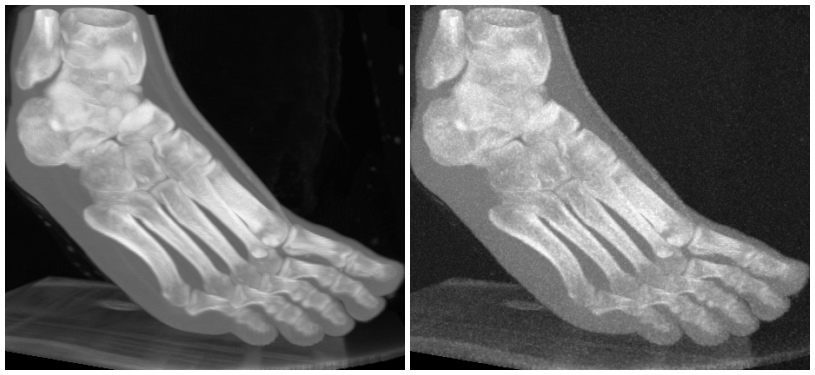
\includegraphics[width=1\textwidth]{figures/3dfoot_vs_noisy.png}
    \begin{tabularx}{1\textwidth}{>{\centering}X>{\centering}X}
        původní volumetrická data (CT chodidla) & volumetrická data s přidaným šumem
    \end{tabularx}
    \caption{Porovnání původních volumetrických dat (výpočetní tomografie chodidla) a volumetrická data s přidaným Gaussovým šumem.}
\end{figure}

Pro testování a porovnání rychlostí filtrů s referenčními filtry jsou připravena umělá volumetrická data s nagenerovaným bílým Gaussovým šumem (ADWR) o rozměrech:
\begin{itemize}
    \item $50\times50\times50$ = 125 000 voxelů
    \item $150\times150\times150$ = 3 375 000 voxelů
    \item $300\times300\times300$ = 27 000 000 voxelů
\end{itemize}
Pro srovnání: 2D obrazová data s FullHD rozlišením ($1920\times1080$) mají 345 600 pixelů a data s 4K rozlišením ($3840\times2160$) mají 8 294 400 pixelů.

\section{Průběh testování a testovací prostředí}
\label{sec:results:testing}
Pro každý filtr (bilaterální filtr a non-local means filtr) jsou provedeny 3 testy:
\begin{enumerate}
    \item Test odfiltrování šumu a porovnání výsledku s referenčním filtrem.
    \item Otestování časové závislosti filtru na počtu použitých vláken pro filtraci.
    \item Porovnání rychlosti filtru s referenčním filtrem na vícero velikostech volumetrických dat.
\end{enumerate}
kde testování probíhá na prostředí s parametry:
\begin{itemize}
    \item operační systém: 64bitový Windows 10 (build 19044)
    \item procesor: Intel(R) Core(TM) i7-7700HQ 2,80GHz (jádra 4/8)
    \item .NET runtime: 6.0.3
    \item python interpret: 3.10.2 [MSC v.1929 64 bit (AMD64)]
    \item verze balíčku Itk: 5.3.0
    \item verze balíčku scikit-image: 0.19.2
\end{itemize}

\section{Bilaterální filtr pro volumetrická data}
\label{sec:results:bl}
Filtrační schopnosti implementovaného 3D bilaterálního filtru lze vidět na obrázku \ref{fig:results:3dbl_vs_noisy}, kde výsledná data po aplikaci filtru mají zřetelně méně šumu, kvůli strategii bilaterálního filtru je kolem hran vidět menší neodstraněný šum. 
Na obrázku \ref{fig:results:3dbl_vs_itk} je porovnání výstupů bilaterálního filtru a referenčního filtru (Itk). Mezi výslednými daty je mírný rozdíl, který není postřehnutelný okem, tyto rozdíly jsou pravděpodobně způsobeny zmenšením vyhledávací oblasti (viz předpočítání vyhledávací oblasti v sekci \ref{subsec:bf:precomupte_bias}).

\begin{figure} [H]
    \centering
    \label{fig:results:3dbl_vs_noisy}
    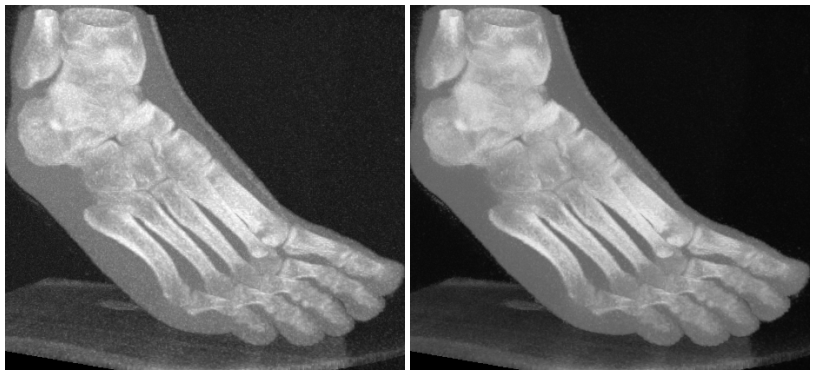
\includegraphics[width=1\textwidth]{figures/3dbl_vs_noisy.png}
    \begin{tabularx}{1\textwidth}{>{\centering}X>{\centering}X}
        zašuměná volumetrická data & 3D bilaterální filtr
    \end{tabularx}
    \caption{Porovnání vstupních zašuměných dat a výsledku po aplikaci 3D bilaterálního filtru s parametry $\sigma_s = 5$ a $\sigma_r = 20$.}
\end{figure}

\begin{figure} [H]
    \centering
    \label{fig:results:3dbl_vs_itk}
    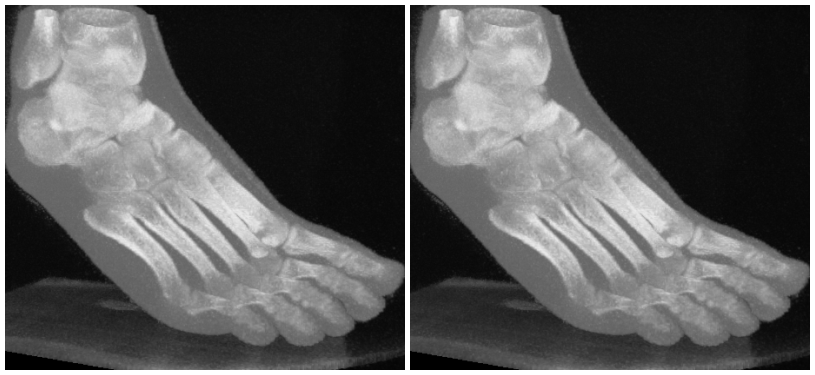
\includegraphics[width=1\textwidth]{figures/3dbl_vs_itk.png}
    \begin{tabularx}{1\textwidth}{>{\centering}X>{\centering}X}
        3D bilaterální filtr & referenční 3D bilaterální filtr -- Itk
    \end{tabularx}
    \caption{Grafické porovnání výstupů bilaterálního filtru a referenčního filtru (Itk) po provedení filtrace se stejnými vstupními parametry: $\sigma_s = 5$ a $\sigma_r = 20$.}
\end{figure}

Na obrázku \ref{fig:results:3dbl_threads} je graf zobrazující časovou závislost implementovaného bilaterálního filtru na počtu použitých vláken při paralelním filtrování. Z grafu je patrný exponenciální pokles efektu počtu vláken na rychlost filtrování a po 4 vláknech má přidání dalších vláken pro filtraci minimální účinek. Nejrychlejšího zpracování dosáhl filtr při filtrování na 7 vláken a při přidání dalšího vlákna (filtrace na 8 vláknech) dosáhl mírně pomalejší výsledku, proto je při porovnání rychlostí bilaterálního filtru s referenčním filtrem použita varianta s~paralelním zpracováním na 7 vláknech.

\begin{figure} [H]
    \centering
    \label{fig:results:3dbl_threads}
    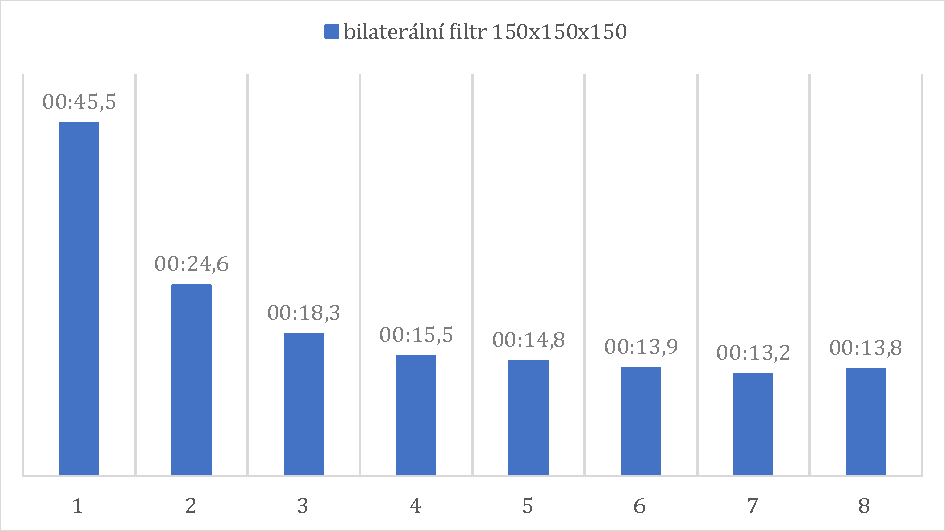
\includegraphics[width=1\textwidth]{figures/3dbl_threads.pdf}
    \caption{Graf zobrazující časovou závislost 3D bilaterálního filtru na počtu vláken při filtrování volumetrických dat o velikosti $150\times150\times150$ a vstupním parametrem $r=12$.}
\end{figure}

Graf na obrázku \ref{fig:results:3dbl} zobrazuje porovnání rychlostí implementovaného 3D bilaterálního filtru a referenčního bilaterálního filtru (Itk). V grafu jsou vidět velké rozdíly v rychlosti filtrů, již při nejmenší velikosti vstupních dat ($50\times50\times50$) trvala filtrace referenčnímu filtru 30 vteřin, což je $75\times$ více než testovanému bilaterálnímu filtru, který stejná data vyfiltroval přibližně za 400 ms. Při filtraci objemnějších dat ($300\times300\times300$) se implementovaný filtr drží v řádech jednotek minut, zatímco filtrace referenčního filtru trvala 37 minut. 

\begin{figure} [H]
    \centering
    \label{fig:results:3dbl}
    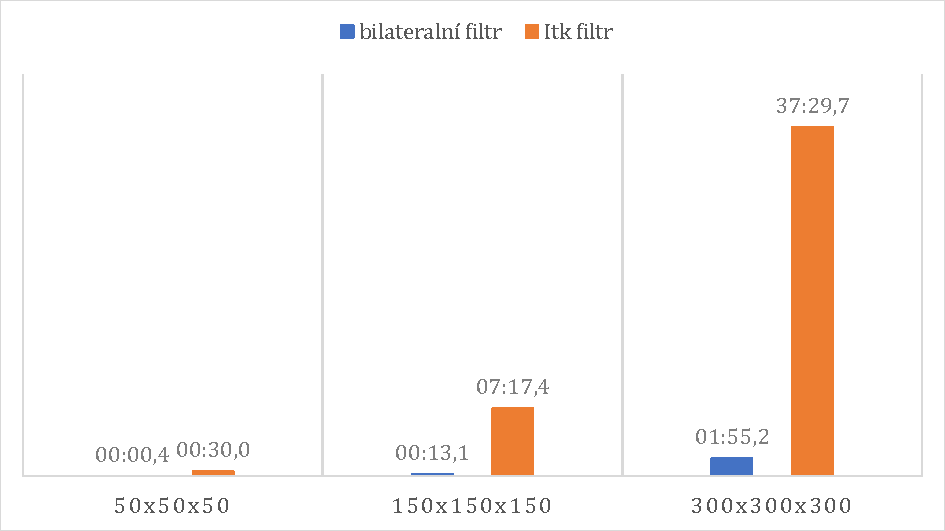
\includegraphics[width=1\textwidth]{figures/3dbl.pdf}
    \caption{Graf porovnávající rychlost 3D bilaterálního filtru (7 vláken) a referenčního filtru (Itk) na různých velikostech volumetrických dat se vstupním parametrem $r=12$.}
\end{figure}

\section{Non-local means filtr pro volumetrická data}
\label{sec:results:nlm}
Filtrační schopnosti implementovaného 3D non-local means filtru lze vidět na obrázku \ref{fig:results:3dnlm_vs_noisy}, kde výsledná volumetrická data po aplikaci filtru nemají téměř žádný šum. Oproti výsledku bilaterálního filtru (obrázek \ref{fig:results:3dbl_vs_noisy}) non-local means filtr odstranil šum i kolem hran.

\begin{figure} [H]
    \centering
    \label{fig:results:3dnlm_vs_noisy}
    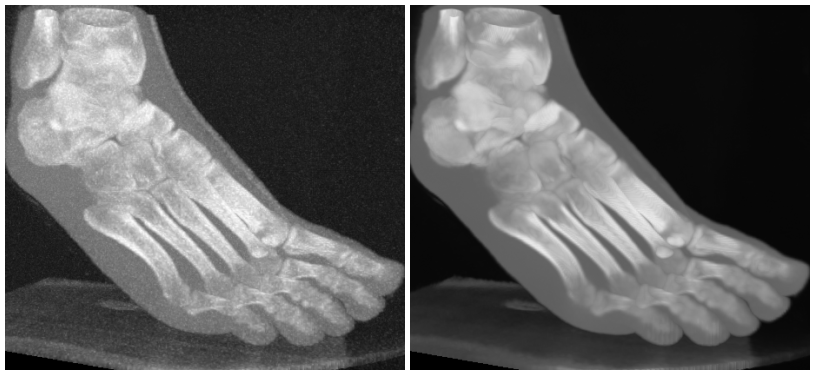
\includegraphics[width=1\textwidth]{figures/3dnlm_vs_noisy.png}
    \begin{tabularx}{1\textwidth}{>{\centering}X>{\centering}X}
        zašuměná volumetrická data & 3D nom-local means filtr
    \end{tabularx}
    \caption{Porovnání vstupních zašuměných dat a výsledku po aplikaci 3D non-local means filtru s navzorkovanou váhovou funkcí (500 vzorků) a vstupními parametry $p=1$, $r=7$ a $h=20$.}
\end{figure}

Na obrázku \ref{fig:results:3dnlm_vs_scikit} je vidět porovnání výstupů implementovaného 3D non-local means filtru a referenčního filtru (scikit-image). Odlišnosti ve výstupech jsou postřehnutelné okem. Protože implementace referenčního filtru také využívá optimalizaci integračním obrázkem, jsou rozdíly pravděpodobně způsobeny jinými optimalizacemi či chybami v implementaci.

\begin{figure} [H]
    \centering
    \label{fig:results:3dnlm_vs_scikit}
    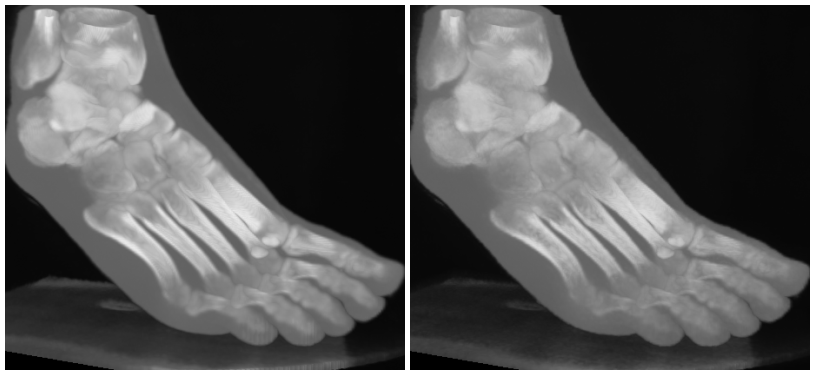
\includegraphics[width=1\textwidth]{figures/3dnlm_vs_scikit.png}
    \begin{tabularx}{1\textwidth}{>{\centering}X>{\centering}X}
        3D non-local means filtr & referenční 3D non-local means filtr -- scikit-image
    \end{tabularx}
    \caption{Grafické porovnání výstupů non-local means filtru (500 vzorků) a referenčního filtru (scikit-image) po filtraci se stejnými vstupními parametry: $p=1$, $r=7$ a $h=20$.}
\end{figure}

\begin{figure} [H]
    \centering
    \label{fig:results:3dnlm_threads}
    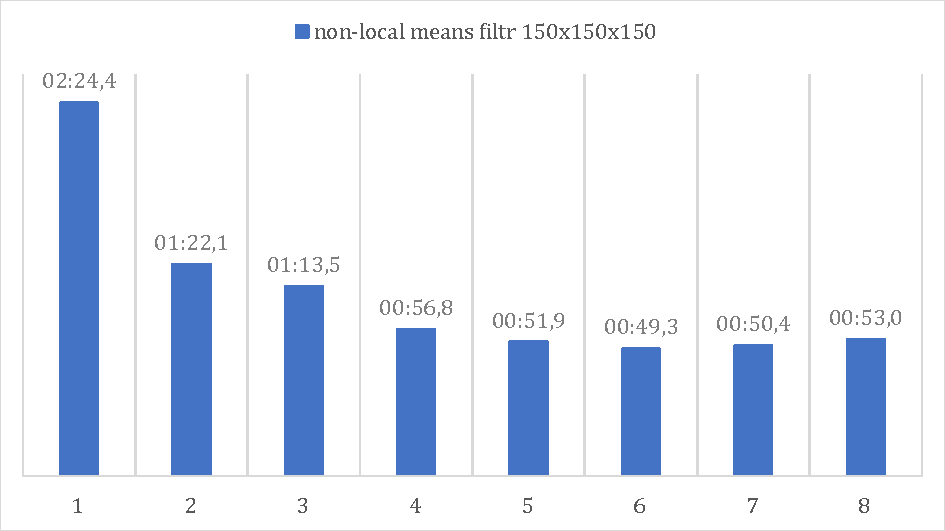
\includegraphics[width=1\textwidth]{figures/3dnlm_threads.pdf}
    \caption{Graf zobrazující časovou závislost 3D nom-local means filtru na počtu vláken při filtrování volumetrických dat o velikosti $150\times150\times150$ a vstupních parametrech $r=7$ a $p=1$.}
\end{figure}

Graf z obrázku \ref{fig:results:3dnlm_threads} zobrazuje časovou závislost implementovaného non-local means filtru na počtu použitých vláken při paralelním filtrování. Z grafu je patrný exponenciální
pokles efektu počtu vláken na rychlost filtrování. Problém horší paralelní zpracovatelnosti non-local means filtru s integračním obrázkem se podepsal v grafu, když počet použitých vláken začal zhoršovat rychlost už od 7 vláken (tj. o 1 vlákno dřív než bilaterální filtr). Pro udržení konzistentnosti s testy bilaterálního filtru je testování rychlosti non-local means filtru prováděno na 7 vláknech. 

Na obrázku \ref{fig:results:3dnlm} je graf, který porovnává rychlost filtrace implementovaného 3D non-local means filtru a referenčního non-local means filtru z knihovny scikit-image. Z grafu je patrné, že implementovaný non-local means filtr je markantně rychlejší než referenční filtr. Protože implementace referenčního filtru nepodporuje paralelní filtraci, porovnání s~paralelně pracujícím filtrem není adekvátní, ale i při porovnání neparalelního zpracování volumetrických dat o velikosti $150\times150\times150$ je implementovaný filtr (02:24,4) $1,7\times$ rychlejší než referenční filtr (04:14,6).

\begin{figure} [H]
    \centering
    \label{fig:results:3dnlm}
    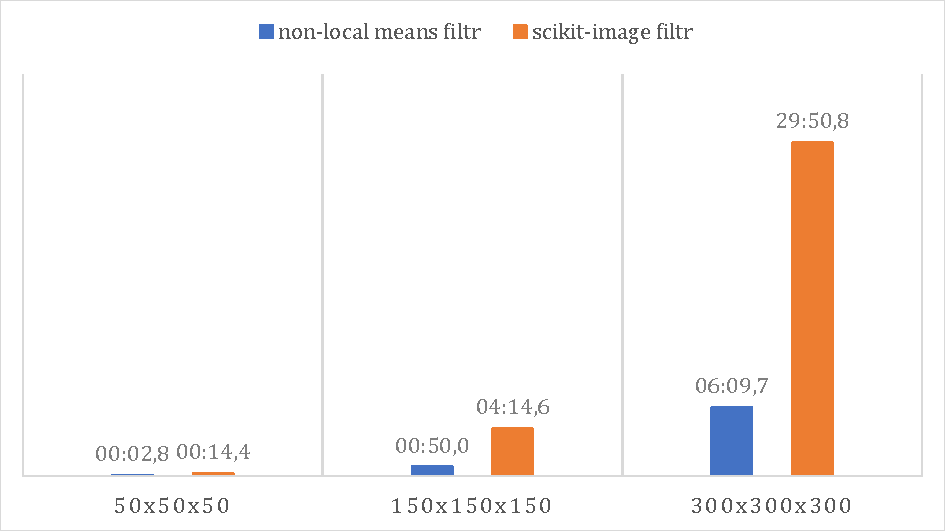
\includegraphics[width=1\textwidth]{figures/3dnlm.pdf}
    \caption{Graf porovnávající rychlost 3D non-local means filtru (7 vláken, 500 vzorků) a referenčního non-local means filtru (scikit-image) na různých velikostech volumetrických dat se vstupním parametry $r=7$ a $p=1$.}
\end{figure}

\chapter{Závěr}
\label{chap:conclusion}
Cílem této práce bylo načerpat znalosti o zpracovávání obrazu, nelineárních filtrech a optimalizacích používaných při filtrování. Následně implementovat zvolené nelineární filtry -- bilaterální filtr a non-local means filtr -- pro 3D obrazová data.

Rychlost a kvalita výsledků implementovaných filtrů ukazují na poměrně kvalitní implementaci filtrů, implementované filtry jsou několikanásobně rychlejší než referenční filtry s~malou nebo téměř žádnou odchylkou výsledků. Využití jazyka C\# pravděpodobně nezhoršilo rychlost filtru, ale naopak napomohlo vytvoření multiplatformní knihovny implementující tyto filtry. Součástí řešení je také ukázková okenní aplikace a konzolová (CLI) aplikace, které demonstrují využití této knihovny. 

S vyšší časovou dotací či lepším rozložením práce by šlo filtry dále optimalizovat použitím SIMD operací či zpracováváním na grafické kartě. Nadstavbou projektu pro další vývoj by mohla být úprava filtrů pro filtraci velkých volumetrických dat, což jsou data s velkými rozměry, případně data, která se celá nevejdou do operační paměti.
Nepřímím rozšířením projektu by také mohla být reimplementace filtrů do známých open source knihoven či aplikací pracujících s volumetrickými daty, případně vývoj aplikace, kteréátyto filtry sama využije. 